\documentclass[preprint,review,12pt]{elsarticle}

\usepackage{amsmath,amssymb}
\usepackage{bm}
\usepackage{booktabs}
\usepackage{graphicx}
\usepackage{url}
\graphicspath{{../firm/figures/}}

\journal{Journal of Computational Physics}

% ----- convenience macros (notation consistent with Basic et al. 2018) -------
\newcommand{\xij}{\mathbf{x}_{ij}}
\newcommand{\Mi}{\mathbf{M}_i}
\newcommand{\Bi}{\mathbf{B}_i}
\newcommand{\oi}{\mathbf{o}_i}
\newcommand{\ow}{\mathbf{o}_{w,i}}
\newcommand{\ri}{\mathbf{r}_i}
\newcommand{\Vi}{\mathbf{V}_i}
\newcommand{\ns}{\mathbf{n}_s}
\newcommand{\Ptan}{\mathbf{P}_{\mathrm{tan}}}
\newcommand{\lap}[1]{\langle\nabla^2 #1\rangle}
\newcommand{\gradop}[1]{\langle\nabla #1\rangle}

\begin{document}

\begin{frontmatter}

\title{A boundary-integrated closure for renormalised meshless operators on elliptic boundary value problems}

\author[a]{Josip Bašić}
\author[b]{Chong Peng}
\address[a]{Faculty of Electrical Engineering, Mechanical Engineering and Naval Architecture, University of Split, 21000 Split, Croatia}
\address[b]{School of Civil Engineering, Southeast University, 211189 Nanjing, China}

\begin{abstract}
A boundary-condition closure for renormalised, least-squares corrected meshless Laplacian
operators is presented. In contrast to treatments that pad the domain with auxiliary particles,
embed it in a level set, or enforce the condition through a weak form, the closure is algebraic
and strong-form: the Neumann and free-surface conditions are folded directly into the discrete
collocation row on a single code path, with the boundary detected from the point cloud and
without tuning parameters. The closure is organised by the condition type. A
Neumann flux enters the right-hand side, and a Dirichlet or Robin value enters the diagonal.
The Neumann flux is imposed by a tangential projection performed in physical space before
renormalisation. A general Gram projector treats non-orthogonal corners exactly, and a
complementary algebraic-ghost closure completes the truncated boundary stencil by reflecting
the neighbours and the node itself across the local reflection group, without extra unknowns.
The free surface is detected from the support-deficiency geometry, and its enforcement
strength cancels to the total kernel weight, which removes any penalty or threshold
parameter. The introduced method, named FIRM (Flux-Integrated Renormalised Meshless), is
verified against analytic ground truths and on irregular-domain Poisson benchmarks, for
regular and highly irregular point clouds in two dimensions, against a second-order
generalised finite difference baseline. The operators are linear-exact on any cloud. The
value closure supraconverges, and the algebraic-ghost closure reduces the Neumann-limited
error by about an order of magnitude and, with the sum normalisation, approaches
second-order convergence at a straight Neumann boundary. Used in a Helmholtz--Hodge
decomposition, the renormalised operators are shown to be consistent for a single decomposition,
the residual divergence equalling the operators' non-adjointness defect and vanishing under
refinement.
\end{abstract}

\begin{keyword}
meshless method \sep boundary conditions \sep renormalised Laplacian \sep
free surface \sep Neumann \sep Poisson equation
\end{keyword}

\begin{highlights}
\item A unified boundary closure integrates Neumann and Dirichlet or Robin conditions into
renormalised meshless operators on one code path.
\item The free surface is detected from the point cloud and enforced without a tuning
parameter, the enforcement strength cancelling to the total kernel weight.
\item Non-orthogonal corners are treated exactly by a general Gram projector applied in
physical space before renormalisation.
\item An algebraic-ghost closure restores Neumann accuracy without extra unknowns, and with
the normalisation it approaches second-order convergence.
\item In a Helmholtz--Hodge decomposition the operators are consistent, the
residual divergence being their non-adjointness defect, but vanishing with refinement.
\end{highlights}

\end{frontmatter}

% =============================================================================
\section{Introduction}
\label{sec:intro}

The numerical solution of elliptic boundary value problems on irregular domains is a
recurring requirement across computational physics. It is especially demanding for meshless
discretisations in which the computational nodes move and the domain boundary is not
represented by a conforming mesh, as in the pressure projection of incompressible free-surface
flow and, more generally, in diffusion, electrostatics, and porous-media seepage on irregular or
evolving domains. In a companion study, a class of renormalised meshless
Laplacian operators was introduced for the Poisson and diffusion
equations~\cite{Basic2018}. These operators are corrected by a local least-squares moment
matrix and remain consistent on highly irregular point arrangements, where the classical
smoothed-particle-hydrodynamics (SPH) Laplacian fails to
converge~\cite{Brookshaw1985,Monaghan1983,Fatehi2011}. Their least-squares correction belongs
to the kernel-gradient renormalisation lineage developed to restore particle
consistency~\cite{Randles1996,Bonet1999,Sigalotti2021}. That study, however, treated the
interior operator and reported Dirichlet and Robin results on prescribed domains only; it left
open how a boundary condition is integrated into the renormalised operator when the boundary is
detected from the cloud rather than prescribed, and how Neumann and free-surface boundaries are
handled on a single code path. The present work closes this boundary gap, and is orthogonal to
the recent extension of the same interior operator to full second-order consistency on
disordered clouds by Asai et al.~\cite{Asai2023}.

Handling boundaries on meshless or otherwise irregular domains has been approached through
several distinct methodological families, which differ less in accuracy than in what each
requires of the geometry. A first family represents the boundary geometrically and embeds it
in a background grid. In the level-set tradition, Gibou and co-workers built
second-order-accurate symmetric discretisations of the Poisson equation on irregular domains
through a ghost-value treatment~\cite{Gibou2002,MinGibou2007,GibouMin2012,Mirzadeh2016},
extended to Robin conditions on implicit interfaces~\cite{Papac2013} and to Voronoi interface
constructions~\cite{Guittet2015}; these methods are accurate and well analysed, but they
require an adaptive Cartesian grid and a level-set description of the geometry. A second family
represents the boundary with auxiliary material. In SPH and ISPH, solid walls and free
surfaces are carried by dummy or mirror particles, repulsive forces, or generalised wall
conditions~\cite{Adami2012,Colagrossi2003,Marrone2011}, by semi-analytical boundary
integrals~\cite{Ferrand2013,Leroy2014,Macia2012}, or by the corrected Laplacians of the
moving-particle semi-implicit family~\cite{Koshizuka1998,Ikari2015,Huang2016,Tamai2017,Ma2016};
these treatments are effective but typically introduce auxiliary particles and a tuning length
or threshold, the free surface in particular being identified by a thresholded density or
kernel-sum criterion. A third family appends the boundary condition as additional algebraic
rows: in the generalised finite difference (GFDM) and finite-pointset (FPM) methods a full
Taylor basis is fitted by weighted least squares and the conditions enter as constraint
rows~\cite{Benito2001,Kuhnert2001,Tiwari2003,Trask2017}, while radial-basis-function finite
differences recover boundary accuracy by adding ghost nodes outside the
domain~\cite{Bayona2010,Fedoseyev2002,Dobravec2024}. Across these families the boundary is paid
for with stored degrees of freedom, a background grid, or a tuning parameter.

A separate line of work injects the boundary condition into the discrete equations
\emph{algebraically}, rather than padding the domain with stored geometry, and three strands may
be distinguished. The first embeds the condition in the trial space \emph{a priori}, so that
every admissible field satisfies it by construction: the R-function method builds
boundary-conforming solution structures from implicit
geometry~\cite{Shapiro2007,ShapiroTsukanov1999}, weighted extended B-splines weight a
tensor-product basis by a boundary distance function~\cite{Hoellig2003}, and the same
construction underlies the exact imposition of boundary conditions in neural and
physics-informed solvers through distance functions~\cite{Lagaris1998,SukumarSrivastava2022}.
The second injects the condition into the variational form rather than the basis: in
element-free Galerkin and related meshfree methods the moving-least-squares shape functions lack
the Kronecker-delta property and so cannot pin nodal values
directly~\cite{Belytschko1994,FernandezMendez2004}, and essential conditions are instead
enforced weakly through Nitsche's method~\cite{Nitsche1971} or a penalty~\cite{Atluri1998}, with
strong-type variants developed more recently~\cite{Hillman2021}. The third does not prescribe a
condition at all but corrects the truncated kernel summation near the boundary so that the
operator stays consistent there, through Shepard normalisation~\cite{Shepard1968}, corrective
and reproducing-kernel formulations~\cite{Chen1999,Liu1995}, and the boundary truncation-error
analysis of Quinlan et al.~\cite{Quinlan2006}; this strand is the closest ancestor of the
renormalised operators used here, though it restores consistency without prescribing the
boundary value or flux. The present closure is algebraic in this sense but differs from all
three: it embeds the boundary condition neither in the trial space nor in a variational form
requiring background integration, but directly into a strong-form collocation row, organised by
condition type, with a Neumann flux entering the right-hand side and a Dirichlet or Robin value
the diagonal of the same row. The boundary is detected from the point cloud, and the closure
carries no tuning parameter.

The contribution of this work is a boundary closure for the renormalised operators
of~\cite{Basic2018} with three properties not jointly provided by the methods reviewed above.
It is \emph{unified}: the interior, the Neumann boundary, the free surface and the contact lines
are assembled by one kernel on a single code path, distinguished only by the boundary-condition
type, a Neumann flux entering the right-hand side and a Dirichlet or Robin value the diagonal of
the same collocation row. It is \emph{geometry-detected}: the free surface is identified from the
support-deficiency geometry of the cloud, without surface particles and without a level set. It
is \emph{parameter-free}: the free-surface enforcement strength cancels to the total kernel
weight, a geometric quantity, and a parameter-free activation leaves the interior nodes
untouched, so the closure introduces no penalty, threshold, or tuning length. A complementary
algebraic-ghost closure removes the accuracy bottleneck of the flux-only Neumann treatment by
completing the truncated boundary stencil with reflected samples that are formed on the fly and
never stored, and so add no unknowns. As a smaller supporting result, the single-sum interior
operator adopted here, which we call the \emph{smooth-naive} operator, bridges the naive and sum
versions of~\cite{Basic2018} through a trace-based normalisation and retains the corrected
summation of the latter in a single neighbour loop. The scope is restricted to the linear
elliptic Poisson problem; applications and extensions are discussed in the conclusions.

The paper is organised as follows. Section~\ref{sec:operators} recalls the renormalised
operators. Section~\ref{sec:closure} derives the boundary closure, comprising the
boundary-condition-by-type principle, the Neumann projection and its corner treatment, the
algebraic-ghost closure, the free-surface detection, and a short consistency remark.
Section~\ref{sec:opresults} reports the pointwise operator-approximation results, including
boundary and corner rows. Section~\ref{sec:bvp} reports the boundary-value-problem benchmarks
and the comparison with the GFDM baseline. Section~\ref{sec:hodge} applies the closure to
the Helmholtz--Hodge decomposition and examines the operators' non-adjointness.
Section~\ref{sec:cost} discusses computational aspects, and Section~\ref{sec:concl} concludes.

% =============================================================================
\section{Meshless operators}
\label{sec:operators}

Three meshless second-derivative operators are used in this work and are set out in this
section in a common notation: the renormalised differencing operator of~\cite{Basic2018},
abbreviated LDD after the Lagrangian differencing dynamics of~\cite{Basic2022}, on which the
boundary closure of Section~\ref{sec:closure} is built; a generalised finite difference (GFDM)
operator used as a second-order baseline; and the second-order renormalised operator
of~\cite{Asai2023}, which we re-express in a kernel-gradient-free form consistent with the
present framework. For a point cloud $\Omega$ with nodal spacing $\Delta$, each node $i$
interacts with neighbours $j$ within a compact support radius $h=\kappa\Delta$ through a kernel
$W_{ij}=W(|\xij|,h)$, where $\xij=\mathbf{x}_j-\mathbf{x}_i$ and $f_{ij}=f_j-f_i$. The kernel
used throughout is the poly6 function
\begin{equation}
  W(r,h)=\max\!\big(0,\;1-q^2\big)^3,\qquad q=r/h,
  \label{eq:kernel}
\end{equation}
with $\kappa=2.5$ by default.

\subsection{Lagrangian Differencing Dynamics (LDD)}
\label{sec:op-ldd}

The renormalised operators of~\cite{Basic2018} consume the kernel weights and renormalise
them, and are therefore kernel-agnostic in the sense made precise below. From the kernel are
formed the
support-deficiency vector $\oi$, the total weight $S_i$, the second-moment renormalisation
tensor $\Mi$ and its inverse $\Bi$,
\begin{align}
  \oi &= \sum_j W_{ij}\,\xij, \label{eq:o}\\
  S_i &= \sum_j W_{ij}, \label{eq:Stot}\\
  \Mi &= \sum_j W_{ij}\,\xij\otimes\xij, \label{eq:M}\\
  \Bi &= \Mi^{-1}. \label{eq:B}
\end{align}
The vector $\oi$ vanishes for symmetric support and points inward near a boundary, and $\Bi$
is symmetric positive-definite whenever $\Mi$ has full rank, which requires at least $d+1$
non-degenerate neighbours. The renormalised gradient is
\begin{equation}
  \gradop{f}_i=\Bi\sum_j W_{ij}\,f_{ij}\,\xij,
  \label{eq:grad}
\end{equation}
which is exact for linear fields on any cloud. For $f=\mathbf a\cdot\mathbf x+b$ the
difference is $f_{ij}=\mathbf a\cdot\xij$, and by the definition of $\Mi$ in Eq.~\eqref{eq:M},
\begin{align}
  \gradop{f}_i
  &=\Bi\sum_j W_{ij}(\mathbf a\cdot\xij)\,\xij \notag\\
  &=\Bi\Big(\sum_j W_{ij}\,\xij\otimes\xij\Big)\mathbf a
   =\Bi\Mi\mathbf a=\mathbf a,
  \label{eq:gradexact}
\end{align}
the renormalisation by $\Bi=\Mi^{-1}$ being precisely what cancels the unbalanced moments of
a truncated support.

The Laplacian is again obtained from a Taylor expansion in which the first-order term is
removed by subtracting the reconstructed gradient. Two members of the renormalised family
derived in~\cite{Basic2018} provide the context. The \emph{naive version} weights each
neighbour by the reciprocal squared distance,
\begin{equation}
  \lap{f}_i^{\mathrm{naive}}=2d\sum_j \frac{W_{ij}}{|\xij|^2}\big(f_{ij}-\xij\cdot\gradop{f}_i\big),
  \label{eq:naive2017}
\end{equation}
which is accurate on regular clouds but is sensitive to close neighbours, since a single near
pair makes $1/|\xij|^2$ large. The \emph{sum version} removes that sensitivity by replacing
the per-neighbour weight with a single self-normalising ratio,
\begin{equation}
  \lap{f}_i^{\mathrm{sum}}=2d\,\frac{\sum_j W_{ij}\,w_{ij}\,f_{ij}}{\sum_j W_{ij}\,w_{ij}\,|\xij|^2},
  \qquad w_{ij}=1-\xij\cdot\Bi\oi,
  \label{eq:sum2017}
\end{equation}
whose denominator is the operator's own action on $\tfrac12|\mathbf x|^2$ and which is
therefore exact for the isotropic quadratic by construction.

The operator introduced here, which we name the \emph{smooth-naive} operator, descends from the
naive form, Eq.~\eqref{eq:naive2017}, by smoothing its normalisation. The per-neighbour factor
$2d/|\xij|^2$ is replaced by a single tensor quantity built from the already-computed
renormalisation tensor,
\begin{equation}
  N_i=\frac{2}{d}\,\mathrm{tr}\,\Bi.
  \label{eq:N}
\end{equation}
It was found that $\mathrm{tr}\,\Bi$ represents the normalisation more smoothly than the
per-neighbour reciprocal, being insensitive to individual close pairs. The factor $2/d$
follows from the spherical-mean identity $\nabla^2 f=\lim_{r\to0}\frac{2d}{r^2}(\bar f_r-f)$
and gives the correct second-derivative magnitude in any dimension, as confirmed by a
three-dimensional constant-Laplacian test in Section~\ref{sec:opresults}. With this
normalisation the corrected second difference reads
\begin{equation}
  \lap{f}_i=N_i\sum_j W_{ij}\big(f_{ij}-\xij\cdot\gradop{f}_i\big).
  \label{eq:lapnaive}
\end{equation}
Because $\gradop{f}_i$ does not depend on $j$, the offset $\sum_j W_{ij}\xij=\oi$ is factored
out of the second term, giving $\sum_j W_{ij}\,\xij\cdot\gradop{f}_i=\oi\cdot\gradop{f}_i$.
Substituting Eq.~\eqref{eq:grad} and using the symmetry of $\Bi$,
\begin{align}
  \oi\cdot\gradop{f}_i
  &=\oi\cdot\Bi\sum_j W_{ij}\,f_{ij}\,\xij \notag\\
  &=\sum_j W_{ij}\,f_{ij}\,(\xij\cdot\Bi\oi),
  \label{eq:collapse}
\end{align}
so the double sum collapses to the single-sum renormalised Laplacian
\begin{equation}
  \lap{f}_i=N_i\sum_j W_{ij}\,f_{ij}\,(1-\xij\cdot\Bi\oi)
           \equiv N_i\sum_j W_{ij}\,f_{ij}\,w_{ij}.
  \label{eq:lap}
\end{equation}

Equation~\eqref{eq:lap} connects the two operators of~\cite{Basic2018}. Its summand
$W_{ij}w_{ij}f_{ij}$ is the numerator of the sum version, Eq.~\eqref{eq:sum2017}, while its
normalisation $N_i$ is the smoothed descendant of the naive weighting,
Eq.~\eqref{eq:naive2017}. The smooth-naive operator therefore retains the corrected,
offset-shifted summation of the sum version, and evaluates it in a single neighbour loop without
the second summation. The three normalisations moreover coincide on isotropic support, where
$w_{ij}\to1$ and $\Mi=\tfrac1d\big(\sum_j W_{ij}|\xij|^2\big)\mathbf I$, giving
\begin{equation}
  N_i^{\mathrm{den}}\equiv\frac{2d}{\sum_j W_{ij}\,w_{ij}\,|\xij|^2}
  \;\xrightarrow{\ \text{isotropic}\ }\;
  \frac{2d}{\sum_j W_{ij}\,|\xij|^2}=\frac{2}{d}\,\mathrm{tr}\,\Bi=N_i,
  \label{eq:Nden}
\end{equation}
the naive, sum and smooth-naive operators all reducing to the same expression on a regular
lattice and differing only under anisotropy. The self-normalising denominator $N_i^{\mathrm{den}}$
of Eq.~\eqref{eq:Nden} is the normalisation of the \emph{sum} operator of~\cite{Basic2018};
applied to the same summand it is retained here as the more accurate variant. Being exact for
$|\mathbf x|^2$, the sum operator is between $8$ and $15\%$ more accurate than the smooth-naive
operator under disorder, with the edge widening as the chaos level grows; the sum-to-smooth-naive
error ratio falls from $1.00$ on a lattice to $0.73$ at chaos $80\%$, as shown in
Section~\ref{sec:bvp}, Fig.~\ref{fig:jitter}. The smooth-naive operator, which avoids the
denominator sum, is the default, and the sum operator is offered as a more accurate refinement.

The correction weight renders Eq.~\eqref{eq:lap} linear-exact on any cloud, including the
truncated rows that occur at a boundary. For $f=\mathbf a\cdot\mathbf x+b$ the field
difference is again $f_{ij}=\mathbf a\cdot\xij$, and
\begin{align}
  \lap{f}_i
  &=N_i\Big[\sum_j W_{ij}(\mathbf a\cdot\xij)-\sum_j W_{ij}(\mathbf a\cdot\xij)(\xij\cdot\Bi\oi)\Big] \notag\\
  &=N_i\big[\mathbf a\cdot\oi-\mathbf a\cdot\Mi\Bi\oi\big]=0,
  \label{eq:lapconsist}
\end{align}
since $\Mi\Bi=\mathbf I$, and the two terms cancel on any support, symmetric or truncated.
Readers interested in the rigorous derivation and the convergence theory of these operators
are referred to~\cite{Basic2018,Lanson2008a,Vila1999}.

It should be noted that Eq.~\eqref{eq:lap} is linear-consistent but not, in general,
second-order consistent on a disordered cloud. On a regular lattice its pointwise truncation
error is $O(\Delta^2)$, whereas under fixed-relative jitter it is $O(1)$ and does not vanish
as $\Delta\to0$. The Poisson solution nonetheless converges, a behaviour known as
supraconvergence, because the $O(1)$ pointwise error is the discrete divergence of a
consistent flux and is damped by the global solve. This behaviour was established
in~\cite{Basic2018}. It frames the accuracy results of the present study and is revisited in
Section~\ref{sec:remark}.

\subsection{Generalised finite differences (GFDM)}
\label{sec:op-gfdm}

As a second-order reference we use a generalised finite difference operator of the
finite-pointset type~\cite{Benito2001,Kuhnert2001,Tiwari2003}. At each node the full quadratic
Taylor basis on the neighbour offsets,
\begin{equation}
  \mathbf p_{ij}=\big[\,x_{ij},\ y_{ij},\ \tfrac12 x_{ij}^2,\ x_{ij}y_{ij},\ \tfrac12 y_{ij}^2\,\big]^\top,
  \label{eq:gfdmbasis}
\end{equation}
is fitted to the field differences $f_{ij}$ by weighted least squares with the same kernel
weights $W_{ij}$, and the Laplacian is read off as the sum of the two pure second-derivative
coefficients,
\begin{equation}
  \lap{f}_i^{\mathrm{GFDM}}=\mathbf e^\top\big(\mathbf P^\top\mathbf W\mathbf P\big)^{-1}
                            \mathbf P^\top\mathbf W\mathbf f,
  \qquad \mathbf e=[\,0,0,1,0,1\,]^\top,
  \label{eq:gfdm}
\end{equation}
with $\mathbf P$ the matrix of basis rows $\mathbf p_{ij}^\top$, $\mathbf W=\mathrm{diag}(W_{ij})$
and $\mathbf f=(f_{ij})_j$. The operator is exact for quadratics and hence second-order
consistent in the interior, on regular and disordered clouds alike, at the cost of a
$5\times5$ local solve in two dimensions and a requirement of at least five well-spread
neighbours; on a regular grid it reduces to the standard five-point stencil. The Neumann flux
is imposed as an exact equality constraint through a local Karush--Kuhn--Tucker saddle system,
in the manner of the finite-pointset constraint row~\cite{Kuhnert2001,Tiwari2003}, and a soft
penalty-flux variant, shown not to converge in Section~\ref{sec:nb}, is referred to as the
penalty form.

\subsection{Second-order operators in LDD form}
\label{sec:op-fi}

The cross-term free LDD operator in Section~\ref{sec:op-ldd} are linear-consistent. 
In a systematic taxonomy of renormalised second-derivative models, Asai et
al.~\cite{Asai2023} identify their \emph{Block Diagonal} operator, equivalent there to the
corrected Laplacian of Schwaiger~\cite{Schwaiger2008} and to the present family, with their
\emph{Naive} variant coinciding with the Taylor-series form of Lian et al.~\cite{Lian2021}.
Full second-order pointwise consistency under disorder is recovered only by their \emph{Full
Inverse} operator, which reinstates the cross-derivative coupling that the block-diagonal
reduction drops, in common with the consistent meshless second-derivative constructions of
Espa\~nol and Revenga~\cite{Espanol2003}, the least-squares moving-particle method of Tamai
and Koshizuka~\cite{Tamai2014}, and the GFDM operator of Section~\ref{sec:op-gfdm}. The
terminology is not uniform across the literature, i.e. what~\cite{Asai2023} call Block Diagonal,
is the variant termed \emph{Full Inverse} in the LDD line of work~\cite{Basic2018,Basic2022}.

This operator attains second order by fitting the full set of second derivatives,
including the cross term, rather than the trace alone. It is written in terms of a
corrected kernel gradient $\widetilde{\nabla} W_{ij}$ and the weighting
$\mathbf r_{ij}\!\cdot\!\widetilde{\nabla} W_{ij}/|\mathbf r_{ij}|^4$. The present framework,
however, never differentiates the kernel of the gradient~\eqref{eq:grad} and the
Laplacian~\eqref{eq:lap}, that use only the scalar weight $W_{ij}$ and the renormalisation $\Bi$. We
therefore apply the idea to an equivalent, kernel-gradient-free form of the operator, expressed in the same
renormalise-by-$\Bi$ idiom as a single weighted least-squares fit. Collect the second
derivatives in $\mathbf u_i=[\,\partial^2_{xx}f,\ \partial^2_{yy}f,\ 2\,\partial^2_{xy}f\,]^\top$
and the quadratic offsets in the basis
$\mathbf s_{ij}=[\,x_{ij}^2,\ y_{ij}^2,\ x_{ij}y_{ij}\,]^\top$. The renormalised
gradient~\eqref{eq:grad} is the stencil $\gradop{f}_i=\sum_j\mathbf c_{ij}f_{ij}$ with
$\mathbf c_{ij}=W_{ij}\Bi\xij$. Removing it from the second difference leaves the second-order
remainder
\begin{equation}
  g_{ij}\equiv f_{ij}-\xij\!\cdot\!\gradop{f}_i=\tfrac12\,\hat{\mathbf s}_{ij}\!\cdot\!\mathbf u_i,
  \label{eq:fi-rem}
\end{equation}
exact for quadratics, in which the basis must be \emph{corrected} for the second-derivative
content that the renormalised gradient itself carries,
\begin{equation}
  \hat{\mathbf s}_{ij}=\mathbf s_{ij}-\mathbf C_i\,\xij,\qquad
  \mathbf C_i=\sum_j W_{ij}\,\mathbf s_{ij}\,(\Bi\xij)^\top.
  \label{eq:fi-corr}
\end{equation}
The term $\mathbf C_i\xij$ is the kernel-gradient-free counterpart of the $R_{(2)}$ correction
of~\cite{Asai2023}; omitting it collapses the fit to the linear-consistent class and the second
order is lost under disorder. The coefficients follow from the weighted normal equations
\begin{equation}
  \mathbf M_i^{\mathrm{FI}}\,\mathbf u_i=2\sum_j W_{ij}\,\hat{\mathbf s}_{ij}\,g_{ij},
  \qquad
  \mathbf M_i^{\mathrm{FI}}=\sum_j W_{ij}\,\hat{\mathbf s}_{ij}\otimes\hat{\mathbf s}_{ij},
  \label{eq:fi-solve}
\end{equation}
a $3\times3$ system in two dimensions, and the Laplacian is the trace
$\lap{f}_i^{\mathrm{FI}}=u_{i,1}+u_{i,2}$. Dropping the cross column of $\mathbf s_{ij}$ recovers
the block-diagonal, linear-consistent operator, and hence Eq.~\eqref{eq:lap}, which is the
equivalence noted above. The construction uses only $W_{ij}$, $\Bi$ and the offsets, with no
kernel derivative; in practice the offsets are scaled by their root-mean-square length to
condition $\mathbf M_i^{\mathrm{FI}}$. This form was verified against the analytic moment
integrals of~\cite{Asai2023}, recovering their uniform-cloud values to the quadrature error,
and against pointwise second-order convergence on disordered clouds.

The present work deliberately retains the original linear-consistent LDD operator and shows that, once
the boundary is closed correctly, it is the boundary closure and not the interior order that
governs the realised accuracy of the solution. The interior operators from this section and the
boundary closure to be introduced are complementary and could be combined, as summarised in
Table~\ref{tab:schemes}.

% =============================================================================
\section{Boundary closure}
\label{sec:closure}

\subsection{Boundary conditions by type}
\label{sec:bytype}

The organising principle of the closure is that the type of the boundary condition, not the
physical quantity it constrains, determines the algebra of its integration into
Eq.~\eqref{eq:lap}. A Neumann condition prescribes a flux $\nabla p\cdot\mathbf n=g$. Since a
flux is a known datum independent of the unknown nodal value, it is moved to the right-hand
side. A Dirichlet or Robin condition prescribes a value, or a value-dependent flux. Since the
constraint involves the unknown nodal value, it contributes to the diagonal self-interaction
term as well as to the right-hand side. Two independent classifications are at work, and the
closure keeps them separate. The \emph{enforcement algebra} just described, flux to the
right-hand side and value to the diagonal, is one axis; the boundary \emph{representation},
prescribed or detected from the cloud, is the other. The two closures derived below are named
for the algebra, a \emph{flux closure} and a \emph{value closure}, while the wall and the free
surface are physical instances of them, the free surface additionally being detected rather than
prescribed. The generalised Robin condition $\nabla p\cdot\mathbf n+\alpha p=\gamma$ unifies the
algebra: the flux closure is the limit $\alpha\to0$ and the value closure the limit
$\alpha\to\infty$, a finite $\alpha$ splitting the datum between the two
(Section~\ref{sec:b3}). The pairing of the wall with a flux and the free surface with a value is
therefore specific to the pressure problem and reverses for the velocity field, where the
no-slip wall is a value closure and the stress-free surface a flux closure
(Section~\ref{sec:concl}). The unified assembled row is
\begin{equation}
  \sum_j W_{ij}\,w_{ij}\,p_{ij}-\sigma_i S_i\,p_i=b_i,
  \label{eq:row}
\end{equation}
with $w_{ij}=1-\xij\cdot\Vi$ and a correction vector $\Vi$ that absorbs the Neumann and
free-surface geometry, derived below. In difference form the sparse matrix and the right-hand
side are assembled as
\begin{align}
  A_{ij} &= W_{ij}\,w_{ij}\quad(j\neq i), \label{eq:Aoff}\\
  A_{ii} &= -\sum_{j} W_{ij}\,w_{ij}-\sigma_i S_i, \label{eq:Adiag}\\
  b_i &= \frac{\nabla^2 p_i}{N_i}+b_{\mathrm{N},i}-\sigma_i S_i\,p_{\mathrm{target}}. \label{eq:rhs}
\end{align}
The source enters normalised by $N_i$. The Neumann flux $b_{\mathrm{N},i}$ is already
normalised and is not divided by $N_i$. The free-surface term contributes $-\sigma_i S_i$ to
the diagonal, Eq.~\eqref{eq:Adiag}, and $-\sigma_i S_i\,p_{\mathrm{target}}$ to the right-hand
side, Eq.~\eqref{eq:rhs}.

\subsection{Flux closure (Neumann) by tangential projection}
\label{sec:wall}

Two flux closures are presented for the Neumann boundary, of which this section presents the
tangential projection scheme. It is linear-exact but imposes only the flux, and the resulting
one-sided normal stencil limits its accuracy, which motivates the algebraic-ghost closure of
Section~\ref{sec:ghost}.

Additional nodes are not generated on the Neumann boundary. 
The modification activates on any node whose
support is truncated by the boundary, within a distance of order $h$. Such a node interacts
with $K$ nearby boundary segments, each with an outward unit normal $\mathbf n_k$, a foot
point $\mathbf x_{f,k}$, and a prescribed flux $g_k$. A tangential projector $\Ptan$ removes
the boundary-normal directions from the reconstruction, and the unresolved normal
contribution is supplied by the known flux. Two projectors are introduced as follows.

The \emph{averaged-normal} projector (referred to as AN) builds a single effective normal
from the boundary normals and projects it out,
\begin{align}
  \mathbf n_{\mathrm{eff}} &= \frac{\sum_k\beta_k\,\mathbf n_k}{\big|\sum_k\beta_k\,\mathbf n_k\big|}, \label{eq:neff}\\
  \Ptan &= \mathbf I-\mathbf n_{\mathrm{eff}}\otimes\mathbf n_{\mathrm{eff}}, \label{eq:AN}
\end{align}
where the proximity weights decay with the distance to the boundary $\delta_{w,k}$,
\begin{equation}
  \beta_k=\frac{\max\!\big(0,\,1-\delta_{w,k}/h_w\big)^2}{\sum_m\max\!\big(0,\,1-\delta_{w,m}/h_w\big)^2}.
  \label{eq:beta}
\end{equation}
The AN projector is exact for a flat boundary and for smooth curved boundaries, but it
introduces an $O(\Delta)$ error at a non-orthogonal corner, where a single averaged normal
cannot span the full normal subspace. The \emph{general Gram projector} (referred to as GGP)
instead removes the entire subspace spanned by the boundary normals. Collecting them as the
columns of $\mathbf N=[\mathbf n_1\,|\cdots|\,\mathbf n_K]$, the Gram matrix and the projector
are
\begin{align}
  \mathbf G &= \mathbf N^\top\mathbf N, \label{eq:gram}\\
  \Ptan &= \mathbf I-\mathbf N\mathbf G^{-1}\mathbf N^\top. \label{eq:GGP}
\end{align}
The projector is symmetric, idempotent and annihilates every boundary normal,
$\Ptan\mathbf n_k=\mathbf 0$, and is therefore exact for arbitrary corner geometry.
Near-parallel boundaries are regularised by $\mathbf G\to\mathbf G+\epsilon\mathbf I$ with
$\epsilon\sim10^{-2}$. For $K=1$ and for orthogonal normals the two projectors coincide, and
for $K=d$ non-coplanar boundaries $\Ptan=\mathbf 0$, so the node is fully enclosed and
determined by the boundary data.

A consequence of the renormalisation is that the projection must be performed in physical
space, on the raw offset $\oi$, before renormalisation by $\Bi$. The projected offset is
formed first and only then renormalised into the correction vector,
\begin{align}
  \ow &= \Ptan\,\oi, \label{eq:ow}\\
  \Vi &= \Bi\,\ow. \label{eq:projorder}
\end{align}
The alternative ordering $\Ptan(\Bi\oi)$ removes a component along $\mathbf n$ rather than the
correct $\Bi\mathbf n$ direction, and the two coincide only if $\mathbf n$ is an eigenvector of
$\Bi$, which does not occur for realistic clouds. Only the project-then-renormalise ordering of
Eq.~\eqref{eq:projorder} preserves linear consistency at the boundary, as is shown next.

With $\Vi=\Bi\ow$ the correction weight becomes $w_{ij}=1-\xij\cdot\Vi$. For a linear field
$f=\mathbf a\cdot\mathbf x+b$, with $f_{ij}=\mathbf a\cdot\xij$, the left-hand side of the
assembled row evaluates, using $\Mi\Bi=\mathbf I$, to
\begin{equation}
  \sum_j W_{ij}\,f_{ij}\,w_{ij}
  =\mathbf a\cdot\oi-\mathbf a\cdot\Mi\Vi
  =\mathbf a\cdot\oi-\mathbf a\cdot\ow
  =\mathbf a\cdot(\mathbf I-\Ptan)\,\oi,
  \label{eq:wallresid}
\end{equation}
a residual that is exactly the part of $\oi$ in the boundary-normal subspace. The closure
cancels it with the prescribed flux placed on the right-hand side,
\begin{equation}
  b_{\mathrm{N},i}=
  \begin{cases}
    g_{\mathrm{eff}}\,(\oi\cdot\mathbf n_{\mathrm{eff}}), & \text{AN},\;g_{\mathrm{eff}}=\textstyle\sum_k\beta_k g_k,\\[2pt]
    (\mathbf N^\top\oi)^\top\mathbf G^{-1}\mathbf g, & \text{GGP}.
  \end{cases}
  \label{eq:bwall}
\end{equation}
That this is the correct cancellation is verified by writing the Gram projector complement as
$\mathbf I-\Ptan=\mathbf N\mathbf G^{-1}\mathbf N^\top$ and noting that, for a linear field,
the vector of nodal fluxes is $\mathbf g=[\,\mathbf n_k\cdot\mathbf a\,]_k=\mathbf N^\top\mathbf a$.
The residual of Eq.~\eqref{eq:wallresid} is then
\begin{equation}
  \mathbf a\cdot(\mathbf I-\Ptan)\oi
  =\mathbf a^\top\mathbf N\mathbf G^{-1}\mathbf N^\top\oi
  =(\mathbf N^\top\oi)^\top\mathbf G^{-1}\mathbf g
  =b_{\mathrm{N},i},
  \label{eq:bwallderiv}
\end{equation}
so $\sum_j W_{ij}f_{ij}w_{ij}=b_{\mathrm{N},i}=\nabla^2 f/N_i+b_{\mathrm{N},i}$ holds, with
$\nabla^2 f=0$, on any truncated support, including a non-orthogonal corner. The reversed
ordering $\Ptan(\Bi\oi)$ would replace $\Mi\Vi=\ow$ in Eq.~\eqref{eq:wallresid} by
$\Mi\Ptan\Bi\oi\neq\ow$, breaking the cancellation. This closure will be referred to as the
\emph{projection closure}.

The projection closure is correct and linear-exact, but it imposes only the first-derivative
flux at the boundary. For nonlinear solutions the normal second derivative
$\partial^2 p/\partial n^2$ is left to one-sided support and is poorly resolved. As the results
of Section~\ref{sec:bvp} show, this makes the Neumann boundary the accuracy-limiter. By the
boundary-layer mechanism of LeVeque~\cite[\S2.12]{LeVeque2007}, an $O(h)$ boundary-row
truncation error sits at a node whose column of the inverse operator is $O(1)$, and is
therefore undamped and pollutes the solution with a large constant. The remedy is to complete
the boundary stencil, which is the subject of the next section.

\subsection{Flux closure (Neumann) by algebraic ghosting}
\label{sec:ghost}

The limitation of the projection closure is removed by stencil completion. Rather than
projecting out the unresolved normal direction, it is filled with image samples, such that
$\partial^2 p/\partial n^2$ becomes a genuine two-sided difference, with the prescribed flux
setting the image values. This is the classical ghost-node, or image-particle,
construction~\cite{Gibou2002,LeVeque2007}, and the contribution here is its packaging for the
renormalised operator without additional unknowns. For a Neumann node $i$ with nearby boundary segments
$\{(\mathbf n_k,\mathbf x_{f,k},g_k)\}$, let $R_k$ denote reflection across the plane through
$\mathbf x_{f,k}$ with normal $\mathbf n_k$, and let the reflection group be the set of
non-empty compositions of the $R_k$. For $K=1$ the group is $\{R_1\}$, and for an orthogonal
corner with $K=2$ it is $\{R_1,R_2,R_2\!\circ\!R_1\}$, the last composition being the corner
double reflection that fills the far quadrant. For a non-orthogonal wedge the group generated
by the two planes is in general infinite, and it is truncated to the single reflections and
the first-order double reflection $R_2\!\circ\!R_1$. This truncation does not reproduce the
exact image set of the wedge, but it is empirically sufficient to restore the symmetry of the
moment tensor $\Mi$ and to recover the convergence reported in Section~\ref{sec:b6}. Every
neighbour $j$ and the node $i$ itself are reflected. A source point $\mathbf x_s$ maps under a composition to
$\mathbf x_s\mapsto\mathbf x_s-2\sigma_k\mathbf n_k$ with
$\sigma_k=(\mathbf x_s-\mathbf x_{f,k})\cdot\mathbf n_k$, and the image carries the
Neumann-consistent value $p_{\mathrm{ghost}}=p_s+\sum_{k}(-2\sigma_k g_k)$. Each image within
$h$ is appended to the support with its kernel weight and is included in $\Mi$, $\oi$ and
$N_i$, which restores near-symmetric support. The completed row may be normalised by either
form of Section~\ref{sec:operators}. The sum normalisation, Eq.~\eqref{eq:Nden}, is found
to restore close to second-order convergence at a straight Neumann boundary and is preferred,
while the smooth-naive form is retained at non-orthogonal corners, as Section~\ref{sec:neustraight}
shows. The Laplacian row then couples the image back to its source node $p_s$, either a
neighbour or $i$, with the standard weight, and the constant flux increment moves to the
right-hand side. Two details are each verified to be necessary.
The self-reflection of $i$ supplies the closest and highest-weight image, its diagonal
contribution cancelling while its flux increment survives on the right-hand side. The corner
double reflection supplies the otherwise missing quadrant. This closure will be referred to as
the \emph{algebraic-ghost closure}. It preserves linear-exactness. For a linear field
$f=\mathbf a\cdot\mathbf x+b$ the flux is $g=\mathbf a\cdot\mathbf n$, and the assigned image
value reproduces the true field at the mirrored point,
\begin{equation}
  p_{\mathrm{ghost}}=f(\mathbf x_s)-2\sigma\,(\mathbf a\cdot\mathbf n)
  =\mathbf a\cdot(\mathbf x_s-2\sigma\mathbf n)+b
  =f(\mathbf x_s-2\sigma\mathbf n)=f(\mathbf x_{\mathrm{ghost}}),
  \label{eq:ghostexact}
\end{equation}
and the completed support is an ordinary, linear-exact renormalised stencil. Unlike the
projection closure, the two-sided support supplies the normal curvature, and the boundary
ceases to be the bottleneck. The reflection plane is exact for straight boundary segments. A
curved boundary is treated by a finely faceted polygon, with a local-plane generalisation left
as future work. The closure is applied only to Neumann nodes. The free surface, the contact
lines, and the interior retain the single code path of Sections~\ref{sec:wall}
and~\ref{sec:surface}.

The ghosts are algebraic and ephemeral. They are formed on the fly within the local neighbour
sum of a single row, contribute to that row's moment tensor and coefficients, and are then
discarded. No ghost particles are stored, no memory is allocated beyond the row-local arrays,
and the global neighbour list is neither extended nor re-searched. This is in contrast to
dummy-particle treatments, which allocate and maintain layers of boundary particles and
enlarge the neighbour search.

\subsection{Value closure (Dirichlet/Robin) and free-surface detection}
\label{sec:surface}

The value closure integrates a Dirichlet or Robin datum into the diagonal of the row, by the
principle of Section~\ref{sec:bytype}. Its showcase is the free surface, a value boundary that
is moreover detected from the cloud rather than prescribed. At the free surface the field
satisfies $p=p_{\mathrm{target}}$, which is zero for a clean surface and $\gamma\kappa$ with
surface tension. No surface particles are placed, and every node with air-side truncation
receives the condition. A Taylor expansion to the surface at a
distance $\delta$ along the outward normal $\ns$ converts the Dirichlet datum into a Robin
form whose flux depends on the unknown nodal value,
\begin{equation}
  \nabla p_i\cdot\ns=\frac{p_{\mathrm{target}}-p_i}{\delta},
  \label{eq:dir2robin}
\end{equation}
which produces the diagonal modification of Eq.~\eqref{eq:row} rather than a pure
right-hand-side term. The surface geometry is obtained from the cloud as the support
deficiency that the Neumann boundary cannot explain, that is, from the projected offset $\ow$,
such that a corner does not contaminate the surface normal. The residual, the outward normal
and the surface distance are
\begin{align}
  \ri &= \Bi\,\ow, \label{eq:ri}\\
  \ns &= -\ri/|\ri|, \label{eq:ns}\\
  \delta &= |\ow\cdot\ns|/S_i. \label{eq:delta}
\end{align}
With these natural estimates the Robin enforcement strength $-(\ow\cdot\ns)/\delta$ cancels to
a geometric quantity. Writing $\ns=-\ri/|\ri|$ and $\ri=\Bi\ow$, the numerator is
\begin{equation}
  \ow\cdot\ns=-\frac{\ow\cdot\ri}{|\ri|}=-\frac{\ow\cdot\Bi\ow}{|\ri|}<0,
  \label{eq:odn}
\end{equation}
the sign being fixed by the positive-definiteness of $\Bi$, since the offset points inward and
the normal outward. The distance estimate is then
$\delta=|\ow\cdot\ns|/S_i=(\ow\cdot\Bi\ow)/(|\ri|\,S_i)$, and the common factor
$(\ow\cdot\Bi\ow)/|\ri|$ cancels between numerator and denominator,
\begin{equation}
  -\frac{\ow\cdot\ns}{\delta}
  =\frac{(\ow\cdot\Bi\ow)/|\ri|}{(\ow\cdot\Bi\ow)/(|\ri|\,S_i)}
  =S_i,
  \label{eq:cancel}
\end{equation}
The enforcement strength is therefore the total kernel weight, which is never singular, is
self-scaling, and is free of any penalty parameter. The free surface is detected, again
without a threshold, from the dimensionless indicator
\begin{equation}
  \lambda_i=|\ri|\,\Delta,
  \label{eq:lambda}
\end{equation}
which is $\approx0$ in the interior and $O(1)$ at the surface, through a smooth activation
$\sigma_i=\sigma(\lambda_i)\in[0,1]$. The cubic smoothstep is recommended,
\begin{equation}
  \sigma_i=S\!\big(3(\lambda_i-\tfrac23)\big),\qquad
  S(t)=\begin{cases}0,&t\le0,\\ 3t^2-2t^3,&0<t<1,\\ 1,&t\ge1,\end{cases}
  \label{eq:smoothstep}
\end{equation}
which is zero for $\lambda_i\le\tfrac23$, leaving the interior nodes untouched, is unity for
$\lambda_i\ge1$, and introduces no parameter. The normal component is then removed in a
regularised manner that avoids normalising $\ri$, and the result is renormalised into the
correction vector and weight,
\begin{align}
  \mathbf o_{*,i} &= \ow-\sigma_i\,\frac{(\ow\cdot\ri)\,\ri}{|\ri|^2+\eta^2}, \label{eq:ostar}\\
  \Vi &= \Bi\,\mathbf o_{*,i}, \label{eq:Vsurf}\\
  w_{ij} &= 1-\xij\cdot\Vi. \label{eq:wsurf}
\end{align}
The diagonal then receives $-\sigma_i S_i$ with the right-hand side receiving
$-\sigma_i S_i\,p_{\mathrm{target}}$, where $p_{\mathrm{target}}$ is evaluated at the
detected surface point $\mathbf x_i+\delta\ns$. The free-surface datum is thereby integrated as
the value-dependent Robin flux of Eq.~\eqref{eq:dir2robin}, its known part entering the
right-hand side and its value-dependent part the diagonal of the same collocation row, just as
the Neumann flux enters the right-hand side. Every boundary condition is in this way recast as a
generalised flux and folded into the operator, which is the sense denoted interchangeably by the
terms ``boundary-integrated'' and ``flux-integrated'' that name the method.

\subsection{Contact lines and the unified equation}
\label{sec:unified}

At a contact line a node is both a Neumann node and a surface node. Because the surface
residual is computed from the projected offset $\ow$, it lies in the boundary-tangential
subspace and the two projections do not interfere. The Neumann projection of
Section~\ref{sec:wall} and the surface removal of Section~\ref{sec:surface} compose into a
single $\mathbf o_{*,i}$ and a single $\Vi$, and Eq.~\eqref{eq:row} is assembled with the
Neumann flux on the right-hand side and the surface term on the diagonal. Interior nodes, with
$\sigma_i=0$ and no boundary, reduce to Eq.~\eqref{eq:lap}. Neumann-only nodes reduce to
Section~\ref{sec:wall}, and surface-only nodes reduce to Section~\ref{sec:surface}. The
single-code-path property is thereby retained for all node classes. A pure-Neumann domain is
singular up to an additive constant and must be closed by a zero-mean constraint rather than a
single-point pin. Any free-surface node, with $\sigma_i>0$, removes the null space
automatically.

\subsection{A remark on consistency and convergence}
\label{sec:remark}

The closures inherit the linear consistency of the interior operator. For
$f=\mathbf a\cdot\mathbf x+b$, the gradient~\eqref{eq:grad}, the Laplacian~\eqref{eq:lap}, the
projection closure~\eqref{eq:bwall} and the algebraic-ghost closure each reproduce the exact
result on any cloud, including truncated and corner rows, which is verified to round-off in
Section~\ref{sec:opresults}. The free-surface cancellation~\eqref{eq:cancel} is an algebraic
identity. As anticipated in Section~\ref{sec:operators}, linear consistency does not imply
second-order pointwise consistency under fixed-relative disorder, and the realised order is
governed by the boundary closure. The value closure supraconverges, whereas the flux-only
Neumann closure, which leaves the normal second derivative one-sided, is the accuracy-limiter
by the undamped-boundary-column mechanism of LeVeque~\cite[\S2.12]{LeVeque2007}. The
algebraic-ghost closure, by supplying that curvature, removes the bottleneck. These statements
are quantified in the following sections. The rigorous consistency and convergence theory of
the underlying operators is given in~\cite{Basic2018,Lanson2008a}.

% =============================================================================
\section{Operator approximation results}
\label{sec:opresults}

The discrete operators were verified against analytic ground truths on regular and scattered
clouds. Throughout, the disorder is measured by the chaos level $c$ of~\cite{Basic2018}. A
node is displaced by a random vector with components in $[-c\Delta/2,\,c\Delta/2]$, and
scattered results are reported as the median over at least twenty random realisations. The
error measure is the normalised root-mean-square error
$\mathrm{Error}=\|\langle f\rangle-f\|_2/\|f\|_2$ of~\cite{Basic2018}.

The renormalised gradient~\eqref{eq:grad} and Laplacian~\eqref{eq:lap} are linear-exact on
every cloud tested, including truncated boundary rows and the non-orthogonal wedge, to
$\sim10^{-15}$ and $\sim10^{-13}$ respectively. The Gram-projector algebra is exact to
$\sim10^{-16}$. The projector $\Ptan$ is idempotent and symmetric, $\Ptan\mathbf n_k=\mathbf 0$
for every boundary normal, AN and GGP coincide for $K=1$ and for orthogonal normals, and three
non-coplanar boundaries give $\Ptan=\mathbf 0$. The Neumann linear consistency
$\sum_j W_{ij}w_{ij}f_{ij}=b_{\mathrm{N},i}$ holds to $\sim10^{-17}$, and the
project-then-renormalise ordering of Eq.~\eqref{eq:projorder} is required, since reversing it
breaks consistency at $O(10^{-3})$ on a jittered cloud. The free-surface
cancellation~\eqref{eq:cancel} holds to round-off, and a hydrostatic, linear Poisson problem
on the wedge tank is recovered to $\sim10^{-14}$ with GGP boundaries. The algebraic-ghost
closure preserves linear-exactness to $\sim10^{-15}$.

The $2/d$ factor of the smooth-naive normalisation, Eq.~\eqref{eq:N}, is pinned by a
three-dimensional constant-Laplacian test, for which the bare $\mathrm{tr}\,\Bi$ form, without
the $2/d$, is in error by a factor of $1.5$. The sum operator, with the denominator
normalisation $N_i^{\mathrm{den}}$ of Eq.~\eqref{eq:Nden}, being exact for the isotropic
quadratic, is between $8$ and $15\%$ more accurate at practical resolutions, with its edge
widening under anisotropy. The sum-to-smooth-naive error ratio falls monotonically from $1.00$
on a lattice to $0.73$ at chaos $80\%$, as shown in Fig.~\ref{fig:jitter}. It is offered as a
refinement, and the smooth-naive operator remains the default for its lower cost.

The pointwise approximation of the operator was examined on the Franke function of
Franke~\cite{Franke1980} over the unit square, in the manner of~\cite{Basic2018}.
Figure~\ref{fig:franke} reports the normalised error of the renormalised Laplacian against
$\Delta$, on a regular lattice and at chaos $30$, $60$ and $90\%$, with two second-order
references, the GFDM operator and the same-family Full-Inverse operator of Asai et
al.~\cite{Asai2023}. On a regular lattice all operators are second-order. Under disorder
the renormalised operator is linear-consistent, and its pointwise order falls with the chaos
level, from $2.0$ on the lattice to about $0.7$, $0.2$ and $0.1$ at chaos $30$, $60$ and
$90\%$, approaching the $O(1)$ truncation error noted in Section~\ref{sec:operators}. The GFDM
operator remains close to second-order throughout, and the Full-Inverse operator, which
augments the present renormalised stencil with the cross-derivative coupling, tracks it to
within plotting accuracy. The two coincide because the lost order is due to the dropped cross
terms and not to the renormalised family itself, so recovering it is a matter of reinstating
those terms, at the cost of a small local solve per node, rather than of leaving the family.
The order of the renormalised operator is
recovered by enlarging the support radius. At chaos $60\%$ the order rises to about $1.0$ when
the support is grown from $2.5\Delta$ to $3.5\Delta$, and to about $1.8$ at $5\Delta$, at the
cost of a wider stencil. The support is nevertheless kept small, because the boundary value
problem solution supraconverges at the smaller support, as Section~\ref{sec:bvp} shows.

\begin{figure}[t]
  \centering
  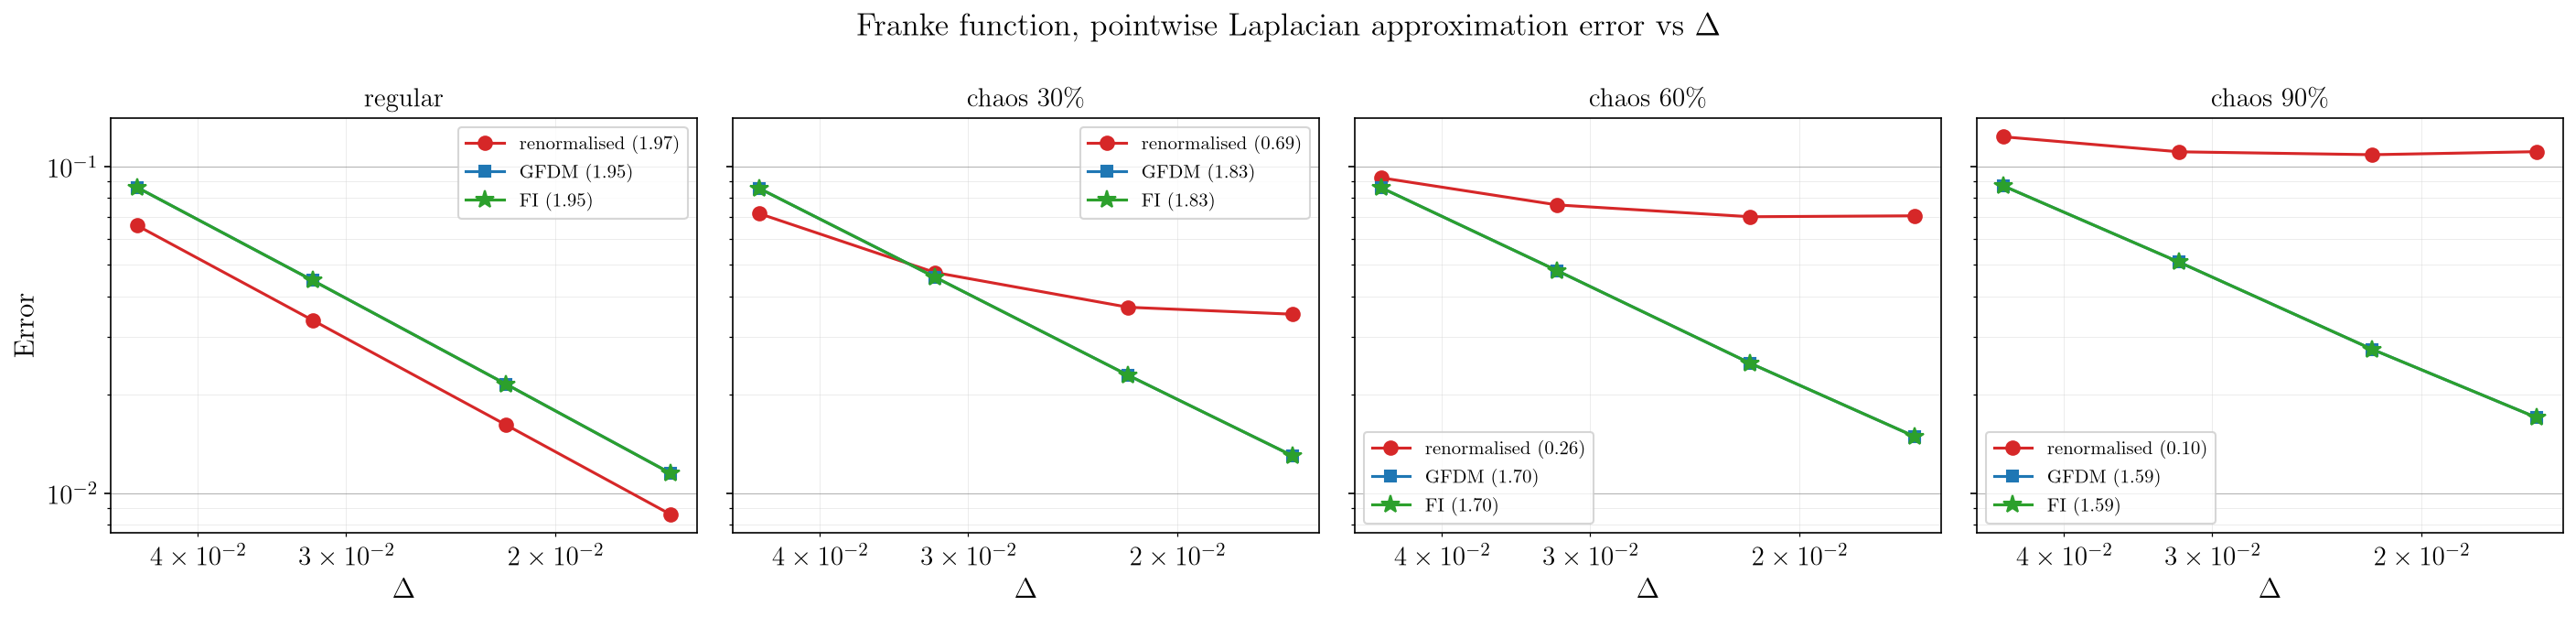
\includegraphics[width=\textwidth]{fig_franke_operator.png}
  \caption{Pointwise Laplacian approximation error of the Franke function against $\Delta$,
  for the renormalised operator and two second-order references, the GFDM operator and the
  same-family Full-Inverse operator of~\cite{Asai2023}, on a regular lattice and at chaos $30$,
  $60$ and $90\%$. On a regular lattice all operators are second-order. Under disorder the
  renormalised operator is linear-consistent and its pointwise order falls with the chaos
  level, whereas the GFDM and Full-Inverse operators, the latter reinstating the
  cross-derivative coupling, remain close to second-order and overlie one another.}
  \label{fig:franke}
\end{figure}

% =============================================================================
\section{Boundary value problem results}
\label{sec:bvp}

The closures were exercised on a set of Poisson benchmarks on irregular domains, extending
the cases of~\cite{Gibou2002,Papac2013} and of~\cite{Basic2018}. Refinement is by halving
$\Delta$, and scattered clouds are tested at chaos $c\in\{30,60,90\}\%$ with median averaging
over at least twenty realisations. The second-order GFDM operator of Section~\ref{sec:op-gfdm}
serves as the meshless baseline throughout, with its Neumann flux imposed by the exact
constraint row and the non-convergent penalty form retained for contrast; for the interior
operator comparisons the same-family Full-Inverse operator of Section~\ref{sec:op-fi} is also
included. The non-convergence of the classical SPH Laplacian on irregular clouds was
established in~\cite{Basic2018} and is not repeated.
Figure~\ref{fig:maps} previews the closures on each domain. It shows the numerical solution
carried on the scattered cloud against the exact-solution contours, for the square with a
Dirichlet condition, the star with a Dirichlet condition, the flower with a Robin condition,
and the wedge tank with Neumann boundaries and a detected free surface.

\begin{figure}[t]
  \centering
  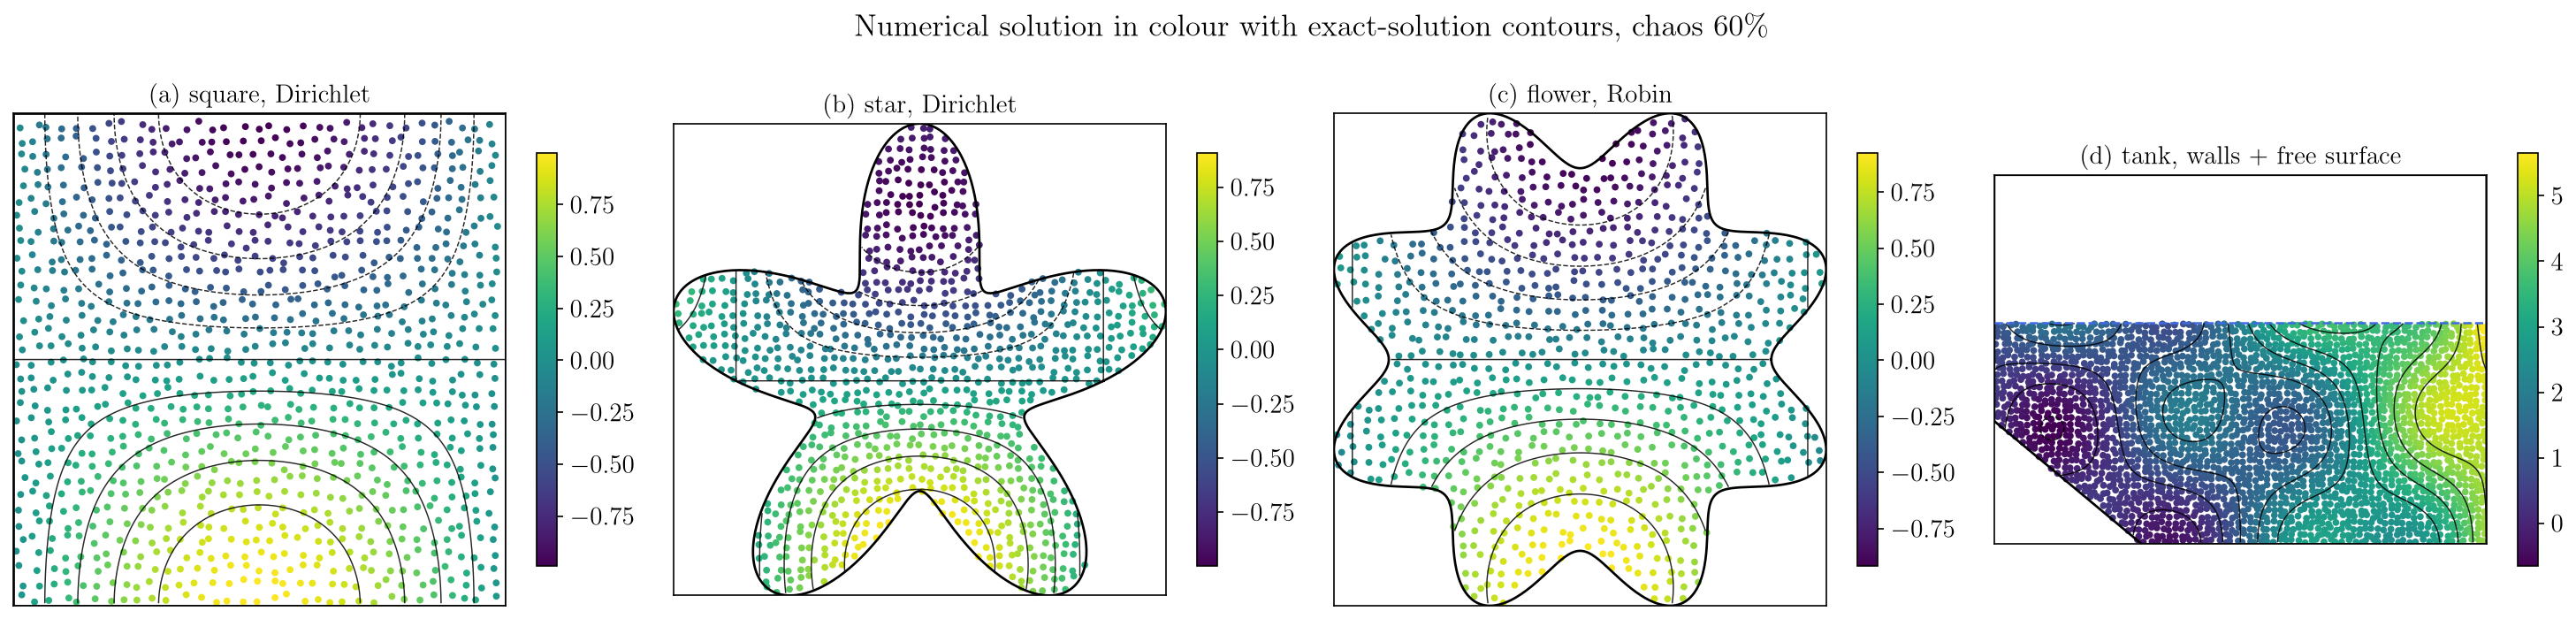
\includegraphics[width=\textwidth]{fig_solution_maps.png}
  \caption{Qualitative solution maps. The numerical solution is carried on the scattered
  cloud, shown in colour, with the exact-solution contours overlaid as lines, at chaos
  $60\%$. From left to right, the square with a Dirichlet condition and the value closure on a
  flat boundary, the star with a Dirichlet condition and the curved value closure, the flower
  with a Robin condition, and the wedge tank with GGP Neumann boundaries, the algebraic-ghost
  closure and a geometry-detected free surface. The contours pass smoothly through the cloud
  in every case, including at the curved and non-orthogonal boundaries.}
  \label{fig:maps}
\end{figure}

\subsection{Square domain with a Dirichlet condition}
\label{sec:b1}

The unit square with a manufactured trigonometric solution and the Franke test
function~\cite{Franke1980} serves as the interior baseline. Figure~\ref{fig:b1} compares the
renormalised closure with the GFDM baseline and the same-family Full-Inverse
operator~\cite{Asai2023} at the three chaos levels. The two second-order operators
retain their pointwise consistency and hold an order near $1.77$ across all
disorder levels, the Full-Inverse and GFDM curves coinciding, whereas the renormalised
operator supraconverges at the linear-consistent ceiling, with an order between $1.4$ and
$1.5$ that degrades only mildly with disorder. The value of the present method does not lie in
the interior order, where a fully second-order operator is more accurate under strong
disorder, but in the boundary closure examined in the following benchmarks, and in its
robustness and absence of tuning; the second-order interior operator and the present boundary
closure are complementary and could be combined.

\begin{figure}[t]
  \centering
  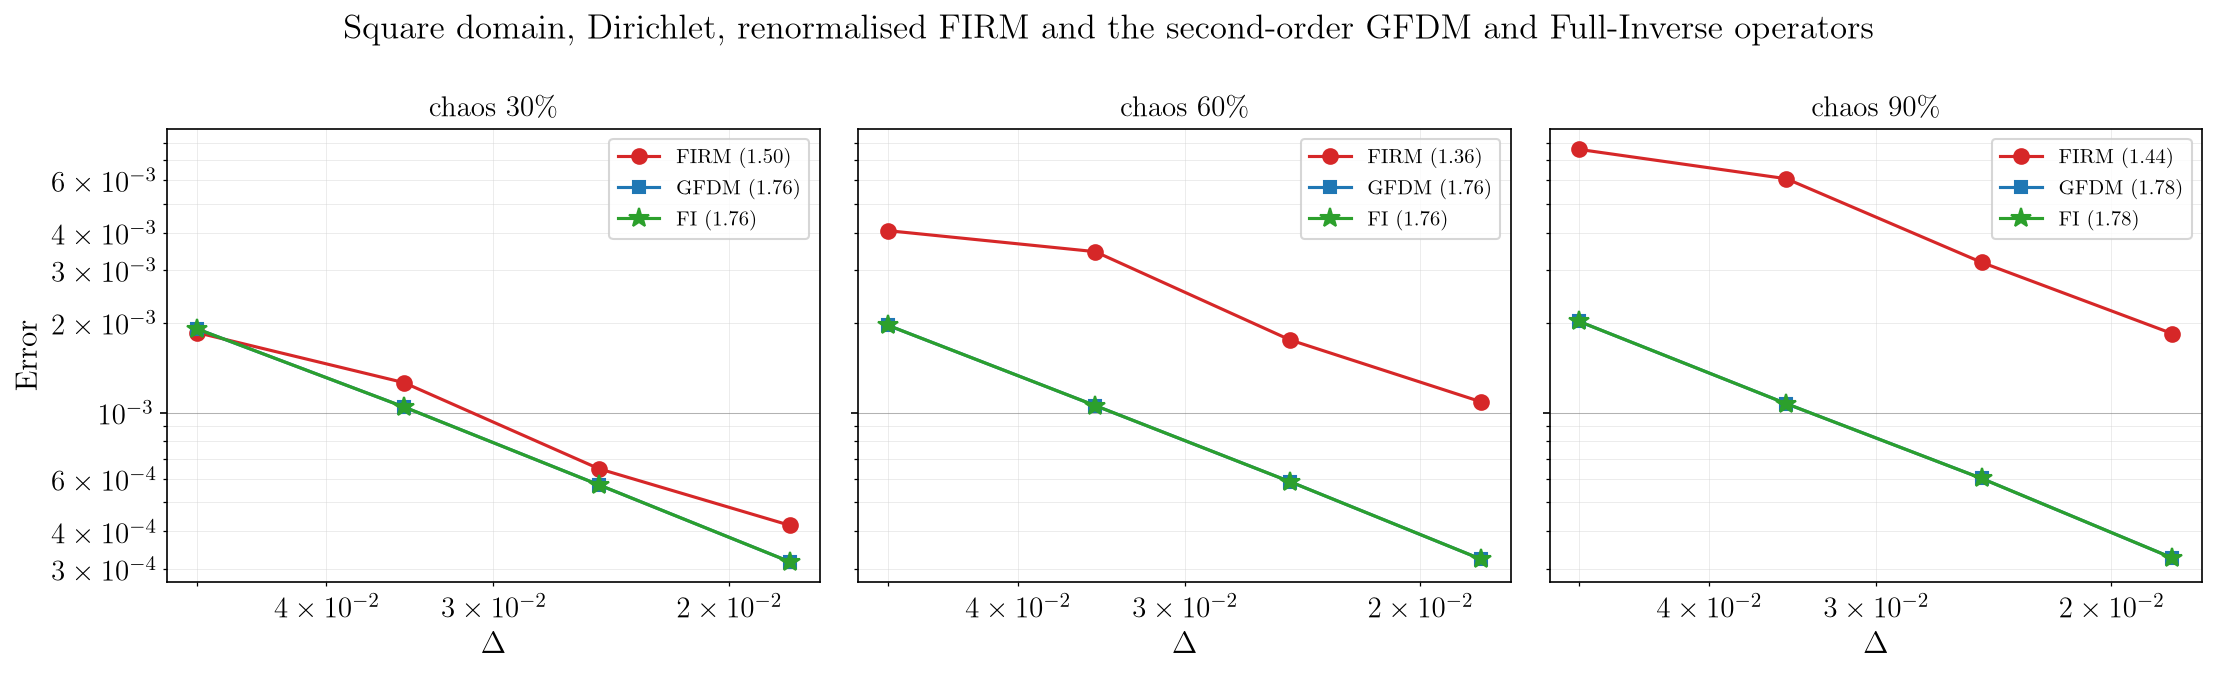
\includegraphics[width=\textwidth]{fig_b1_dirichlet.png}
  \caption{Square domain with a Dirichlet condition and a trigonometric solution. Normalised
  RMSE against $\Delta$ for the renormalised closure FIRM and two second-order baselines, the
  GFDM operator and the same-family Full-Inverse operator of~\cite{Asai2023}, at chaos $30$,
  $60$ and $90\%$. The renormalised operator supraconverges at an order of about $1.4$ to
  $1.5$, while the GFDM and Full-Inverse operators retain their second-order interior order of
  about $1.8$ and coincide.}
  \label{fig:b1}
\end{figure}

\subsection{Neumann boundaries by projection, algebraic ghost and GFDM constraint row}
\label{sec:nb}

The all-Neumann unit box, closed by a zero-mean constraint, isolates the Neumann treatment.
Table~\ref{tab:neumann} and Figure~\ref{fig:neumann} compare four closures, namely the FIRM
projection closure, the FIRM algebraic-ghost closure, the GFDM exact constraint row and the
GFDM penalty form. The two flux-only closures, FIRM projection and the GFDM constraint row,
behave alike. Both impose the flux exactly yet leave the normal second derivative one-sided,
and both converge only slowly, at order about $0.9$, and carry a large error constant, with
the Neumann term dominating the pure-Neumann error. The penalty form is indistinguishable from
the constraint row, which confirms that a soft flux is not the deficiency. The algebraic-ghost
closure, which completes the stencil, is about eight times more accurate at the finest
resolution, $4.7\times10^{-3}$ against $3.9\times10^{-2}$. The all-Neumann box is singular up to
an additive constant, so its per-closure order is dominated by the null-space handling and is
not a reliable rate. The convergence rate is therefore reported on the well-posed wedge tank of
Section~\ref{sec:b6}, where the ghost closure lifts the Neumann-region order from about $1.0$ to
between $1.3$ and $1.8$, so the Neumann region converges at roughly the rate of the interior. It
should be noted that the algebraic-ghost
closure outperforms the GFDM constraint row here because completing the stencil supplies the
curvature that an exactly imposed flux does not. A high-order Neumann treatment would instead
require the staggered KKT construction of Trask et al.~\cite{Trask2017}, which is noted as
future work.

\begin{table}[t]
  \centering
  \caption{All-Neumann box at chaos $30\%$, normalised mean-removed RMSE against $\Delta$. The
  two flux-only closures, FIRM projection and the GFDM constraint row, stall at a large
  constant set by the one-sided normal curvature, and the penalty form is indistinguishable from
  the constraint row. The FIRM algebraic-ghost closure is about an order of magnitude lower. The
  box is singular up to an additive constant, so its per-closure order is set by the null-space
  handling and is not reported here. The convergence rate is reported on the well-posed wedge
  tank in Section~\ref{sec:b6}. Seed-averaged values from the verification suite.}
  \label{tab:neumann}
  \begin{tabular}{lcccc}
    \toprule
    $\Delta$ & FIRM projection & FIRM ghost & GFDM constraint & GFDM penalty \\
    \midrule
    0.050 & $1.05\times10^{-1}$ & $1.1\times10^{-2}$ & $1.22\times10^{-1}$ & $1.22\times10^{-1}$ \\
    0.035 & $7.2\times10^{-2}$ & $1.6\times10^{-2}$ & $8.8\times10^{-2}$ & $8.8\times10^{-2}$ \\
    0.025 & $6.0\times10^{-2}$ & $2.2\times10^{-3}$ & $6.7\times10^{-2}$ & $6.7\times10^{-2}$ \\
    0.018 & $3.9\times10^{-2}$ & $4.7\times10^{-3}$ & $4.7\times10^{-2}$ & $4.7\times10^{-2}$ \\
    \bottomrule
  \end{tabular}
\end{table}

\begin{figure}[t]
  \centering
  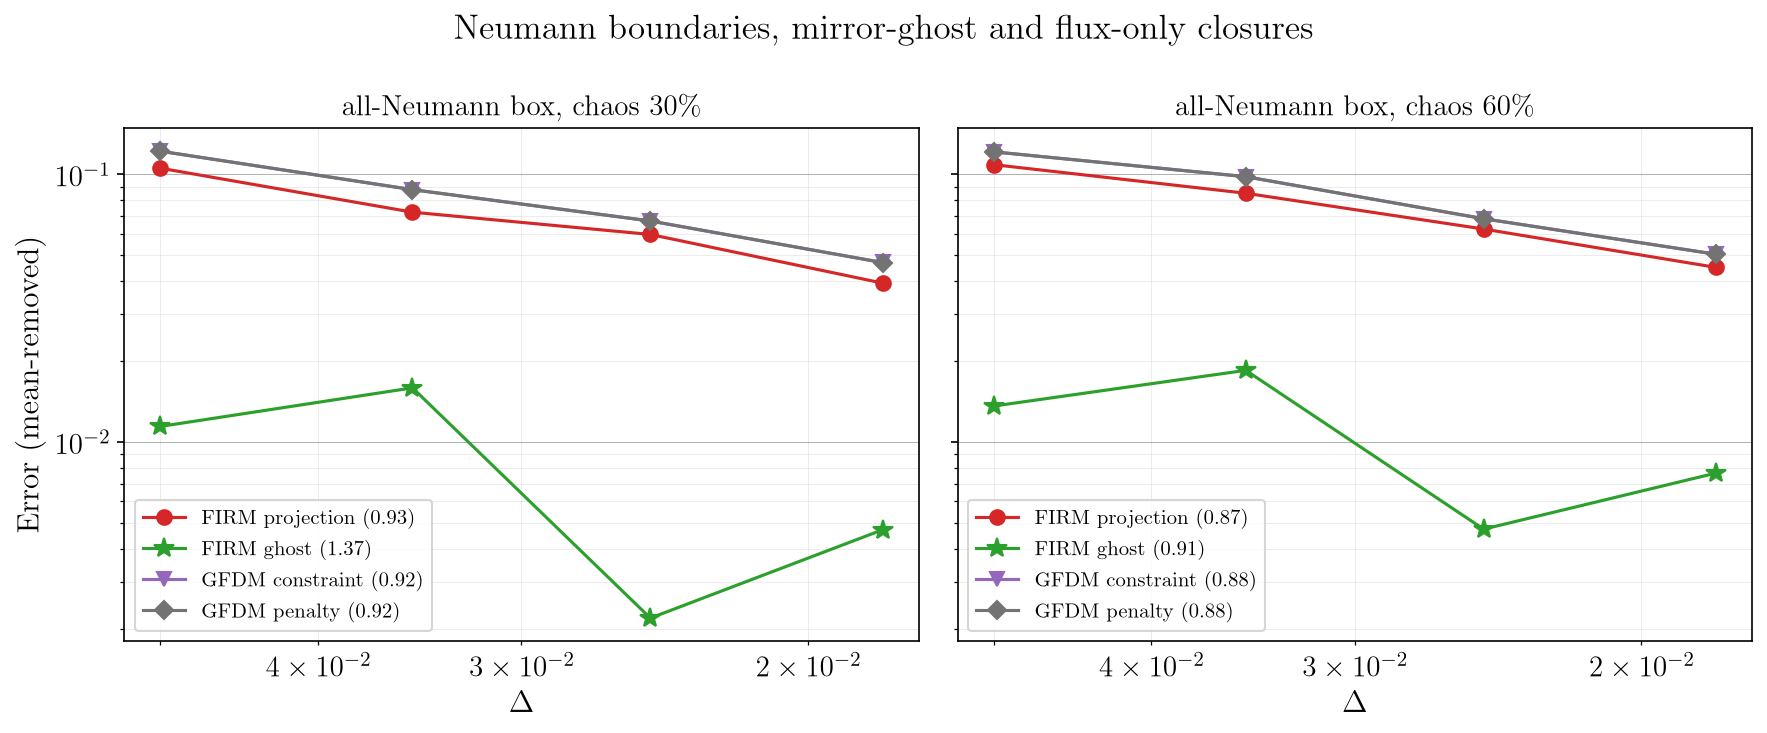
\includegraphics[width=\textwidth]{fig_neumann_baseline.png}
  \caption{Neumann boundaries on the all-Neumann box. The FIRM algebraic-ghost closure is
  compared against the flux-only closures, namely FIRM projection, the GFDM constraint row and
  the GFDM penalty form, at chaos $30\%$ and $60\%$. Completing the boundary stencil restores
  accuracy that an exactly imposed flux alone does not.}
  \label{fig:neumann}
\end{figure}

\subsection{Normalisation of the ghost closure}
\label{sec:neustraight}

The order to which the algebraic-ghost closure converges depends on the normalisation of the
completed row. This is isolated on a square with a single straight Neumann edge at $y=0$ and
Dirichlet conditions on the other three edges, which is well-posed and free of the corner
truncation of Section~\ref{sec:ghost}. Figure~\ref{fig:neustraight} reports the error on the
Neumann edge against $\Delta$. The projection closure converges at order about $0.8$. The ghost
closure with the smooth-naive normalisation, Eq.~\eqref{eq:N}, improves the constant by an order
of magnitude but its error plateaus, at an order of about $1.4$. The ghost closure with the sum
normalisation, Eq.~\eqref{eq:Nden}, which is exact for $|\mathbf x|^2$, removes the plateau and
continues to converge, at an order of about $1.8$, approaching second order. On the completed,
near-symmetric support the two forms differ only through the residual anisotropy, and the sum
form, by reproducing the curvature of $|\mathbf x|^2$ exactly, supplies the normal second
derivative that the smooth-naive form leaves biased. The sum normalisation is therefore preferred
for the ghost closure on straight and smoothly curved Neumann boundaries. At a non-orthogonal
corner the rate is instead capped by the truncated reflection group of Section~\ref{sec:ghost},
where the more robust smooth-naive form is retained, as Section~\ref{sec:b6} shows.

\begin{figure}[t]
  \centering
  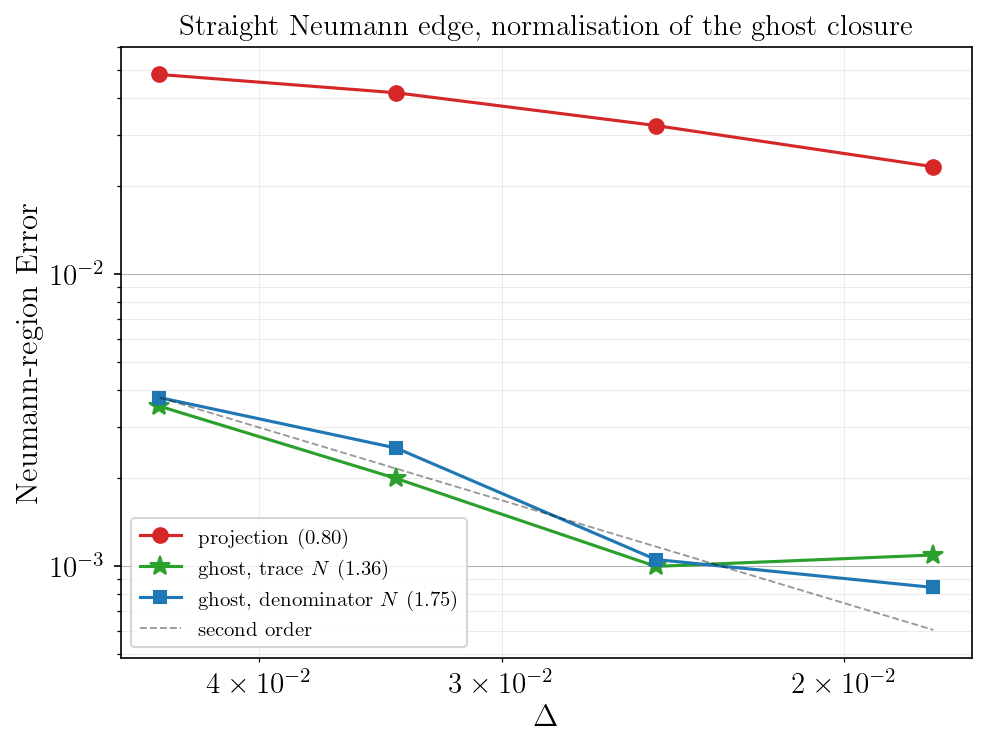
\includegraphics[width=0.62\textwidth]{fig_neumann_straight.png}
  \caption{Straight Neumann edge, error on the edge against $\Delta$. The projection closure
  converges at order about $0.8$. The ghost closure with the smooth-naive normalisation plateaus
  at order about $1.4$, whereas the ghost closure with the sum normalisation
  approaches second order. Seed-averaged over sixteen realisations.}
  \label{fig:neustraight}
\end{figure}

\subsection{Star domain with Dirichlet and Neumann conditions}
\label{sec:b2}

A star-shaped domain $r(\theta)=0.5+0.2\sin5\theta$, after~\cite{Gibou2002}, with a
trigonometric manufactured solution, exercises the closures on a curved boundary. The
boundary is finely faceted, and the residual faceting error is held below the solution error.
For the Dirichlet condition the value closure of Section~\ref{sec:surface} is used with the
local boundary normal and distance, and it supraconverges at order about $1.85$, in line with
the GFDM baseline at about $1.4$. For the Neumann condition the projection closure is again the
limiter at order about $0.8$, while the algebraic-ghost closure improves both the constant and
the order to about $1.7$. The GFDM constraint row tracks the projection closure at about $0.9$,
as on the box. Figure~\ref{fig:b2} collects the curves.

\begin{figure}[t]
  \centering
  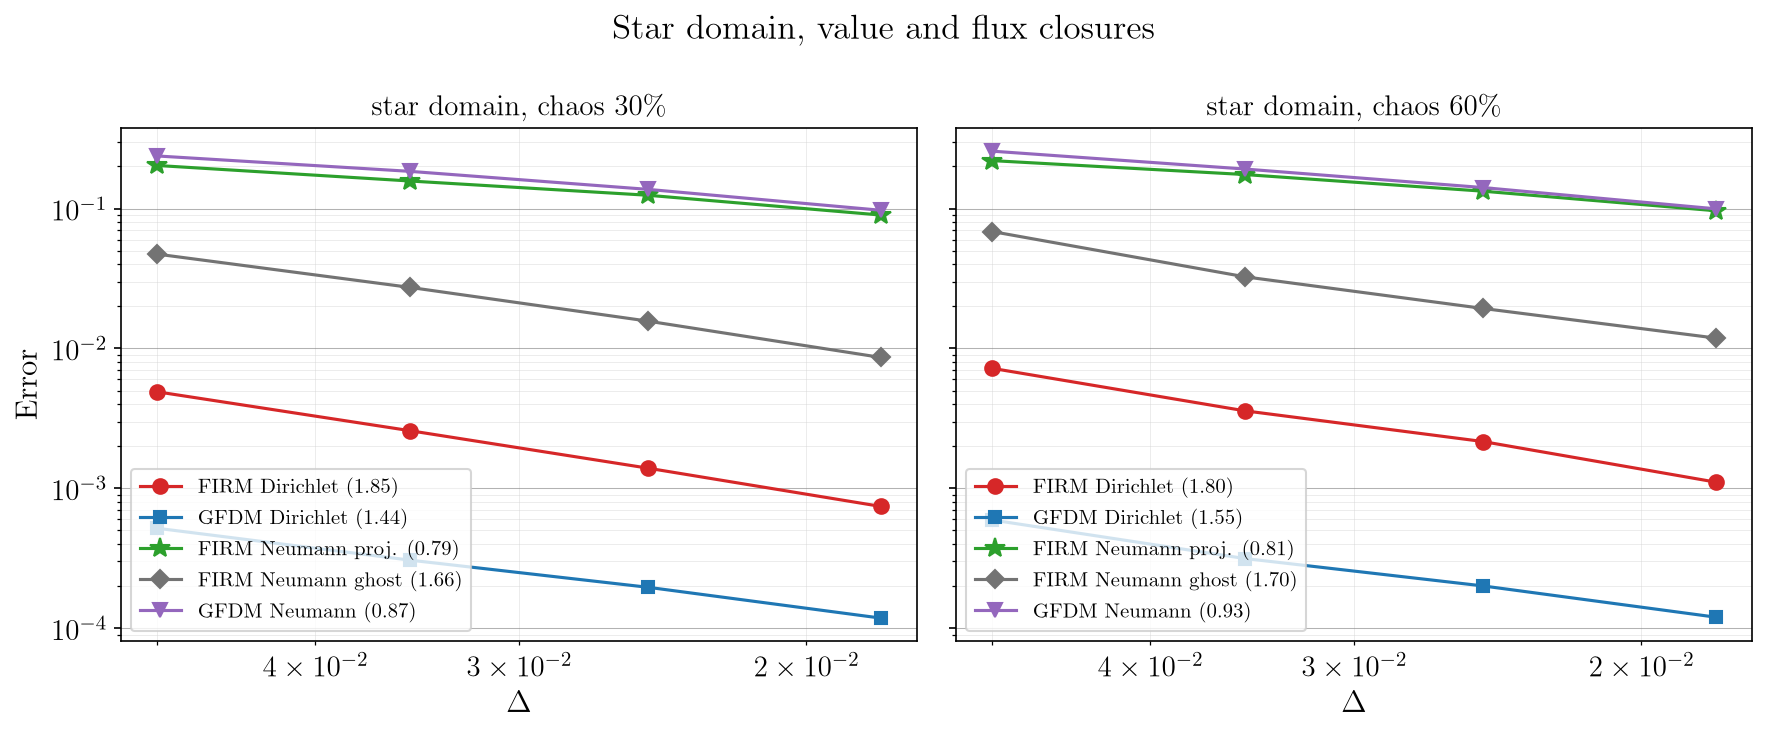
\includegraphics[width=\textwidth]{fig_b2_curved.png}
  \caption{Star domain. The value closure for the Dirichlet condition and the flux closures
  for the Neumann condition on a curved boundary, at chaos $30\%$ and $60\%$. The Dirichlet
  value closure supraconverges, and among the Neumann closures the algebraic ghost is the most
  accurate.}
  \label{fig:b2}
\end{figure}

\subsection{Flower domain with a Robin condition}
\label{sec:b3}

A flower-shaped domain with a Robin condition $\partial u/\partial n+\alpha u=f$ exercises the
value-dependent flux closure. The boundary value, which is unknown, is eliminated by the local
Taylor relation along the perpendicular foot, $u(\mathbf x_f)=u_i+\delta\,\partial u/\partial n$.
Substituting this into the Robin condition $\partial u/\partial n+\alpha\,u(\mathbf x_f)=f$ and
solving for the normal flux gives
\begin{equation}
  g=\frac{\partial u}{\partial n}=\frac{f-\alpha u_i}{1+\alpha\delta},
  \label{eq:robin}
\end{equation}
whose known part $f/(1+\alpha\delta)$ enters the flux right-hand side exactly as in
Eq.~\eqref{eq:bwall}, while the value-dependent part $-\alpha u_i/(1+\alpha\delta)$ is linear
in the unknown and moves to the diagonal, contributing $\alpha/(1+\alpha\delta)$ times the
geometric weight $(\mathbf N^\top\oi)^\top\mathbf G^{-1}\mathbf 1$. Equation~\eqref{eq:robin}
recovers the Neumann closure as $\alpha\to0$, where $g\to f$ and there is no diagonal term,
and the Dirichlet value closure as $\alpha\to\infty$, where $g\to(f/\alpha-u_i)/\delta$, and it
remains linear-exact for straight segments. The realised order rises from about $0.9$ at chaos
$30\%$ to about $1.1$ at chaos $90\%$, consistent with a flux-type closure, as shown in
Figure~\ref{fig:b3}.

\begin{figure}[t]
  \centering
  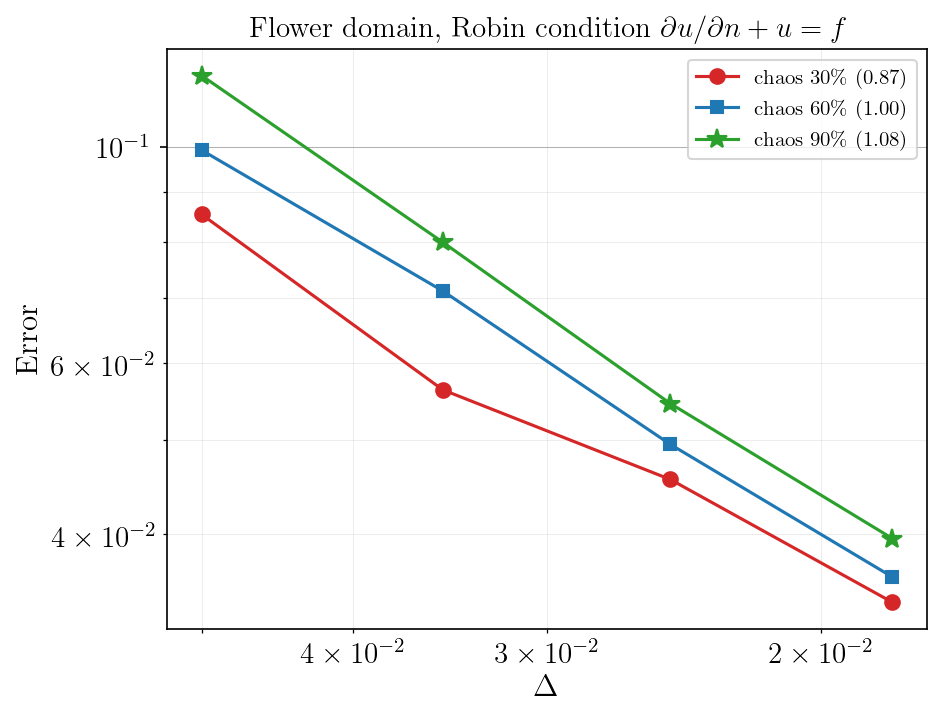
\includegraphics[width=0.6\textwidth]{fig_b3_robin.png}
  \caption{Flower domain with the Robin condition $\partial u/\partial n+u=f$. Normalised RMSE
  against $\Delta$ at chaos $30$, $60$ and $90\%$.}
  \label{fig:b3}
\end{figure}

\subsection{Free-surface detection from the cloud}
\label{sec:b5}

This benchmark treats the upper boundary of a polygonal tank as an unknown free surface,
detected from the cloud by the indicator $\lambda_i$ and the smoothstep activation of
Section~\ref{sec:surface}, with no surface particles and no prescribed geometry. The detector
separates the interior from the surface. The interior indicator is $\lambda^{(90)}\approx0.2$,
well below the activation threshold $\tfrac23$. The outermost surface ring has
$\lambda\approx0.7$ to $0.9$. The interior activation is identically zero, with no false
activation at any tested resolution or disorder, and the recovered surface normal agrees with
the true vertical to within a few percent. The geometry-detected closure tracks a
prescribed-boundary reference. The surface-region error of the detected, or natural, closure
converges at order about $1.5$, close to but slightly below the prescribed, or exact,
reference at about $2.2$, with no tuning parameter. Figure~\ref{fig:b5} shows the detected
activation field on the tank and the detected-versus-prescribed convergence. For comparison,
the rational activation $\sigma=\lambda^2/(\lambda^2+c^2)$ with a fixed $c$ over-activates the
interior at strong disorder, whereas the smoothstep remains pinned at zero, which motivates
the parameter-free choice.

\begin{figure}[t]
  \centering
  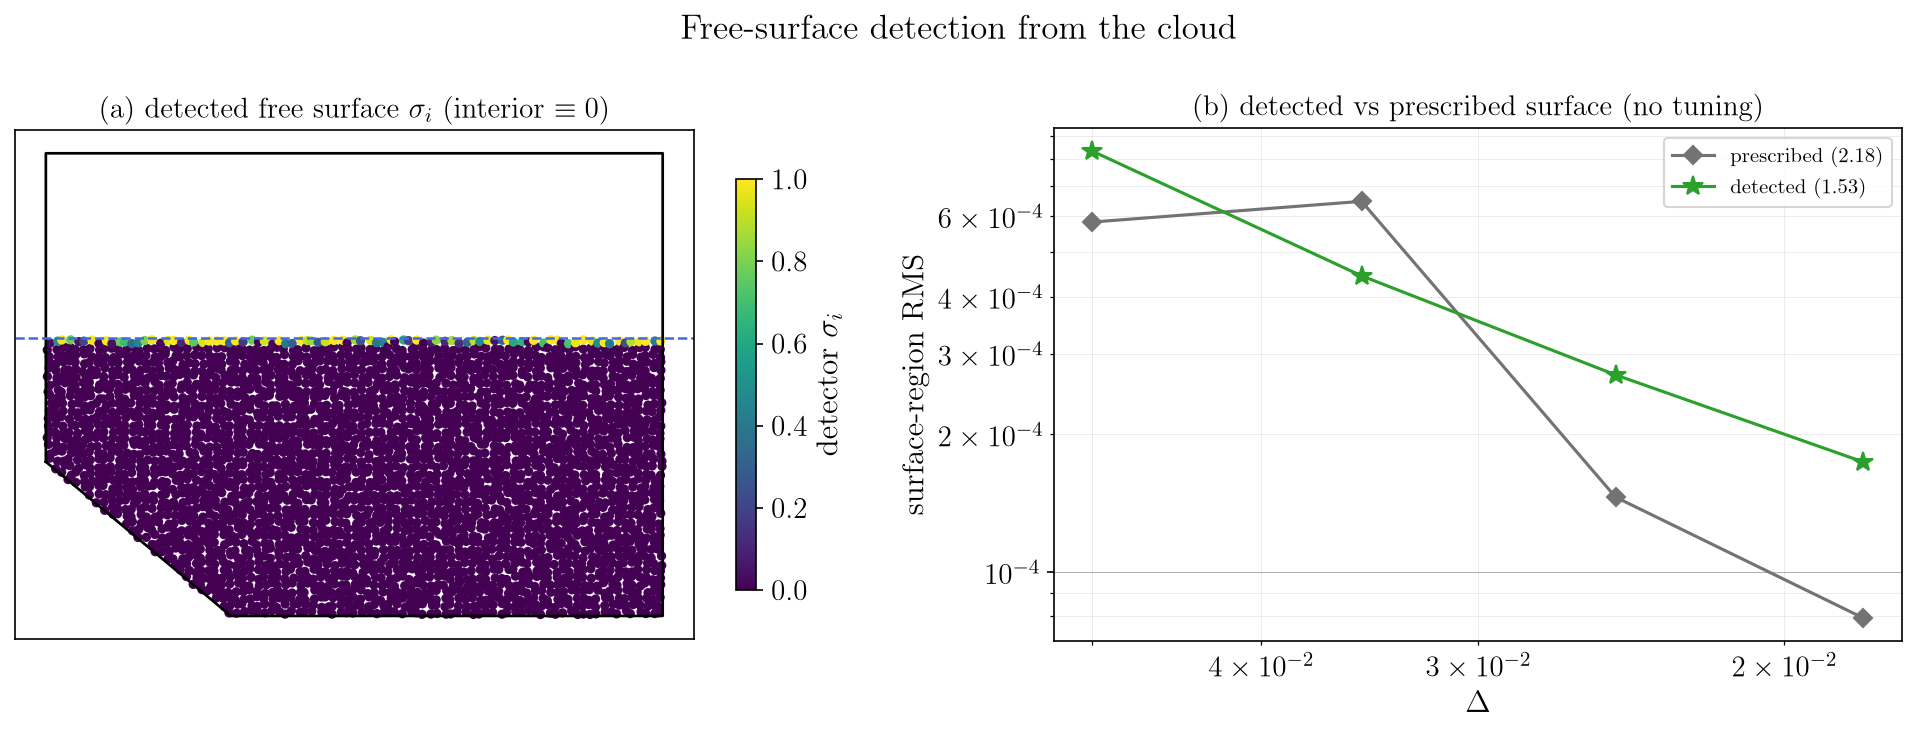
\includegraphics[width=\textwidth]{fig_b5_surface.png}
  \caption{Free-surface detection from the cloud. (a) The geometry-detected activation
  $\sigma_i$ on the jittered tank, identically zero in the interior and rising to unity at the
  surface. (b) The detected, or natural, surface closure converges on top of the prescribed,
  or exact, reference, with no tuning parameter.}
  \label{fig:b5}
\end{figure}

\subsection{Non-orthogonal wedge with a free surface}
\label{sec:b6}

A polygonal tank with a non-orthogonal slant-and-floor wedge and a free surface combines all
closures on a complex manufactured field $p^\star=\sin\pi x\cos\pi y+0.3(x^2+y^2)$. At the
wedge the GGP projector is exact for a linear field, with relative error $\sim10^{-14}$,
whereas AN leaks $O(\Delta)$, with relative error $\sim3\times10^{-2}$, as predicted in
Section~\ref{sec:wall}. For the complex field the error concentrates on the boundaries and the
wedge and vanishes towards the free surface, so the Neumann region is the accuracy-limiter
under the projection closure, where it converges at order about $1.0$. Replacing the projection
closure by the algebraic-ghost closure reduces the Neumann-region error by about an order of
magnitude, from $1.0\times10^{-2}$ to $7.6\times10^{-4}$ at the finest resolution, and lifts the
Neumann-region order to about $1.3$ over the full range and about $1.8$ over the fine range. The
Neumann region thereby converges at roughly the rate of the interior and the Dirichlet
boundary, of about $1.4$ to $1.8$, rather than at the reduced rate of the projection closure,
so it is no longer the limiter. The errors are seed-averaged over six realisations. The corner
double reflection and the self-reflection are both required for this. These results are shown
in Figure~\ref{fig:convergence}, and the error field in Figure~\ref{fig:errorfield}.

\begin{figure}[t]
  \centering
  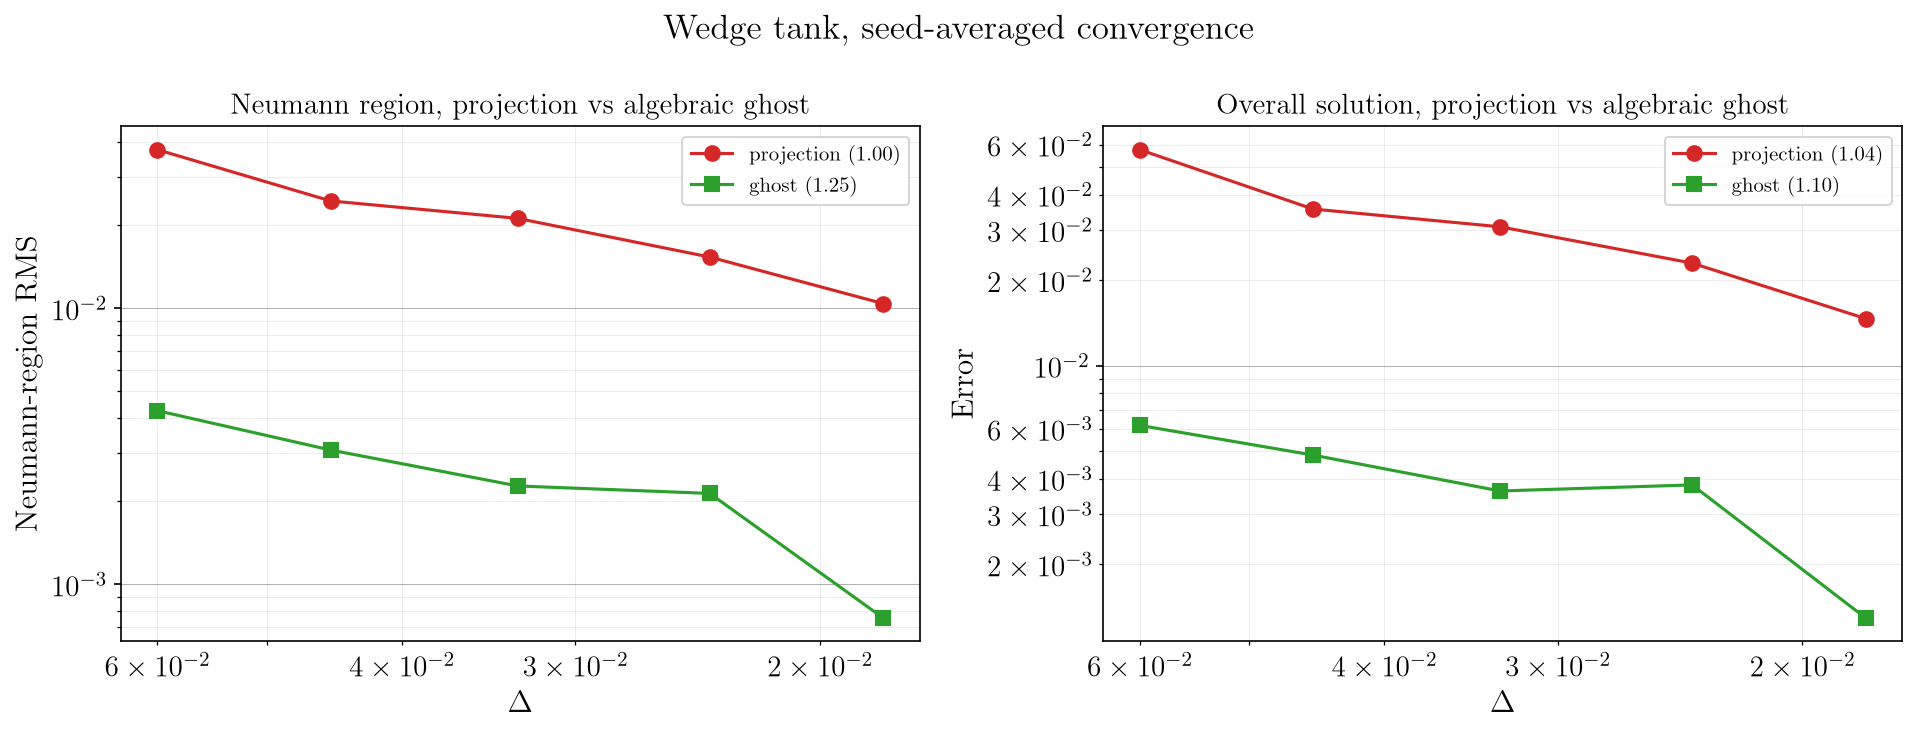
\includegraphics[width=\textwidth]{fig_convergence.png}
  \caption{Wedge tank, seed-averaged over six realisations. Left, the Neumann-region RMS for
  the projection and algebraic-ghost closures. Right, the overall error for the two closures.
  The ghost closure lowers the Neumann-region error by about an order of magnitude and lifts its
  order to roughly the interior rate, so the Neumann region is no longer the limiter.}
  \label{fig:convergence}
\end{figure}

\begin{figure}[t]
  \centering
  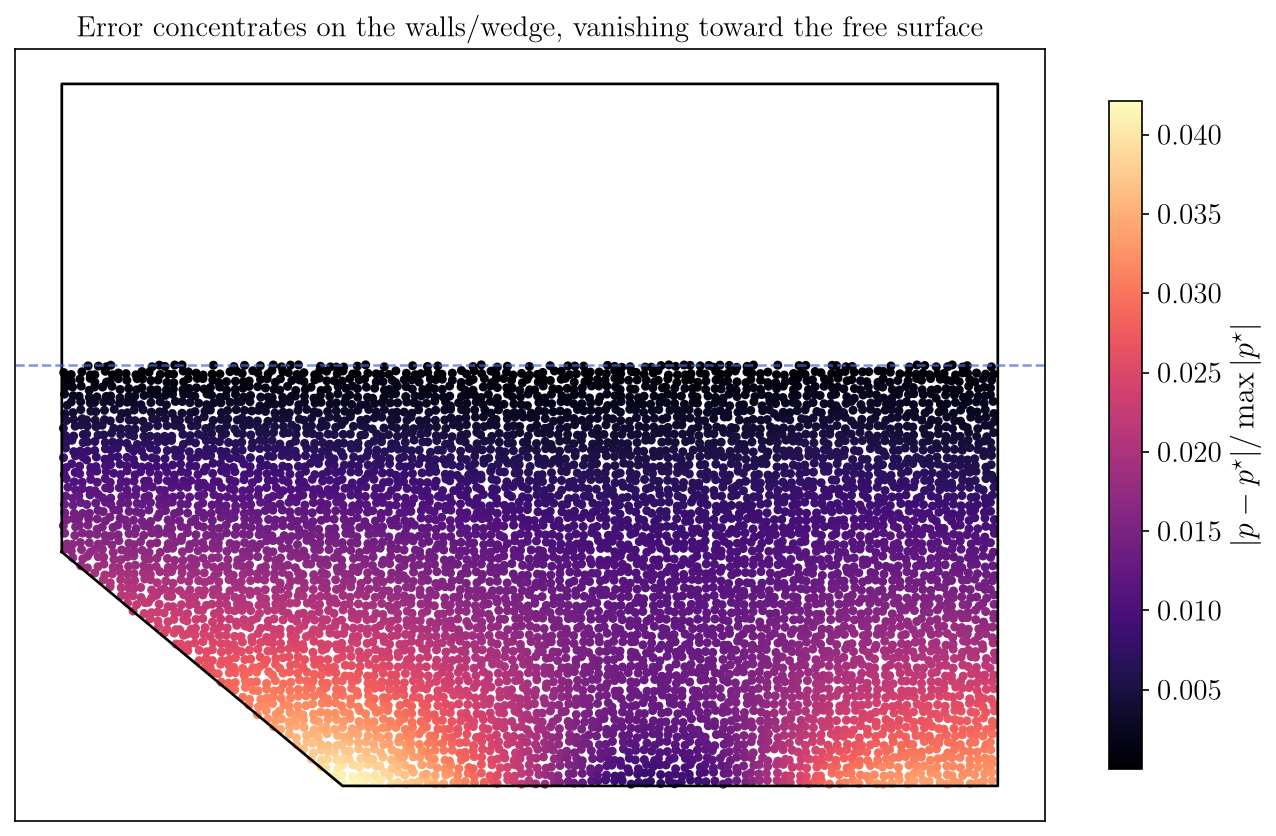
\includegraphics[width=0.7\textwidth]{capstone_error_field.png}
  \caption{Wedge tank. Pointwise error $|p-p^\star|$ for the GGP closure with the prescribed
  surface at the finest resolution. The error concentrates on the boundaries and the wedge and
  vanishes toward the free surface, which identifies the Neumann closure as the limiter.}
  \label{fig:errorfield}
\end{figure}

\subsection{Kernel, support radius and disorder robustness}
\label{sec:b7}

The operators are kernel-agnostic in that linear-exactness holds for the poly6 $(1-q^2)^3$,
the spiky $(1-q)^3$ and the Wendland-C2 kernels at every support radius. The solution accuracy
is not. At matched support the poly6 kernel uses its neighbours most evenly and is the most
accurate at small support. For example, at $h=2.0\Delta$ the Poisson error is
$2.3\times10^{-3}$ for poly6 against $6.6\times10^{-3}$ for the spiky kernel. The concentrated
spiky kernel is competitive only at $h\gtrsim2.5\Delta$, where the small-support advantage is
lost. The default $h=2.5\Delta$ is robust, with about fifteen interior and at least four
boundary neighbours at chaos $60\%$. A smaller $h\in[2.0,2.25]\Delta$ is viable for
quasi-uniform clouds, with the algebraic-ghost closure relieving the boundary-truncation
constraint, while $h\le2.2\Delta$ hits the two-dimensional rank floor of three neighbours under
strong disorder and becomes noisy. Across chaos $0$ to $80\%$ the operators remain
linear-exact, the condition number of $\Mi$ rises smoothly from $1.9$ to about $6$ while $\Mi$
stays invertible, the smoothstep activation never false-triggers the interior, and the
denominator-normalisation edge widens with anisotropy. These trends are collected in
Figures~\ref{fig:kernel} and~\ref{fig:jitter}.

\begin{figure}[t]
  \centering
  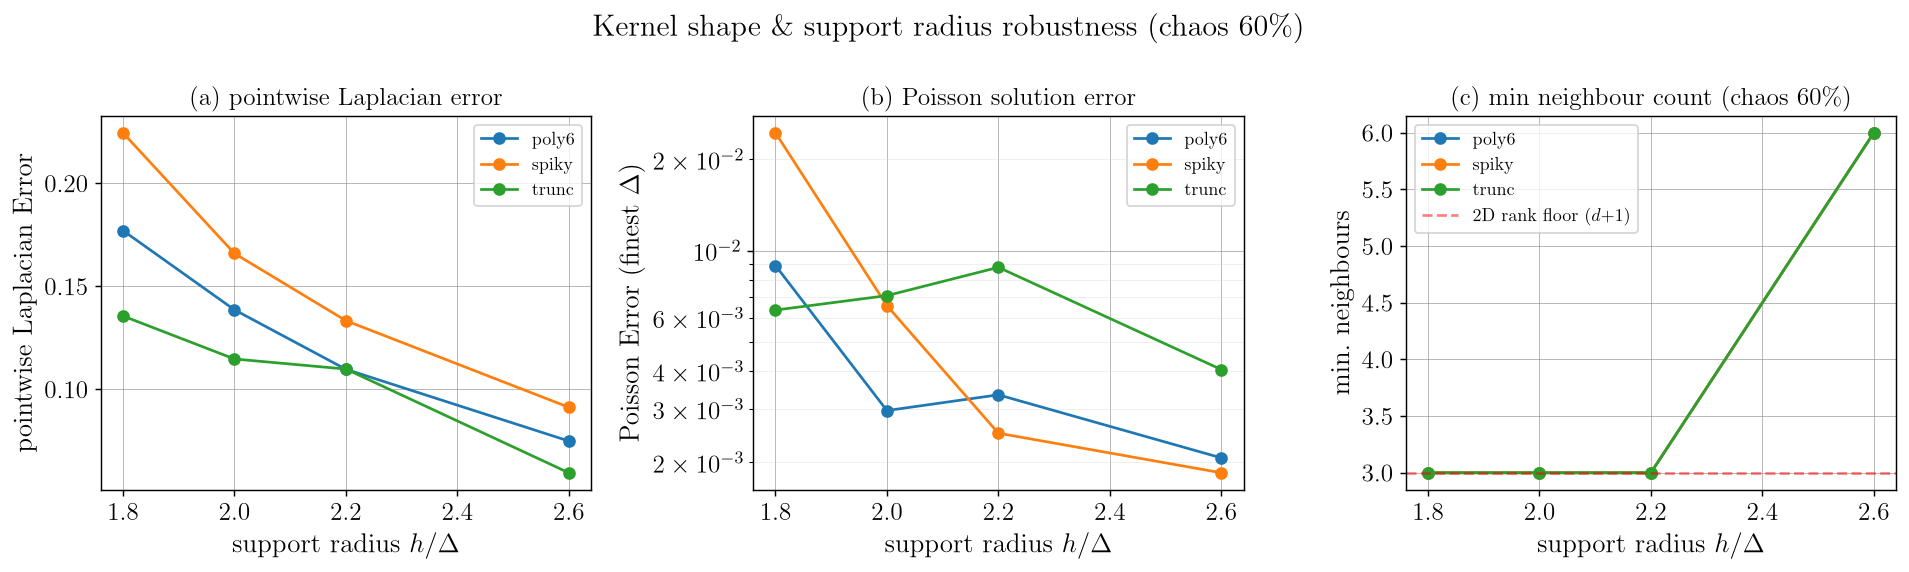
\includegraphics[width=\textwidth]{fig_kernel_radius.png}
  \caption{Kernel and support radius at chaos $60\%$. (a) Pointwise Laplacian error. (b)
  Poisson solution error, lowest and most robust for poly6 at small support. (c) Minimum
  neighbour count, showing the two-dimensional rank floor at small radius.}
  \label{fig:kernel}
\end{figure}

\begin{figure}[t]
  \centering
  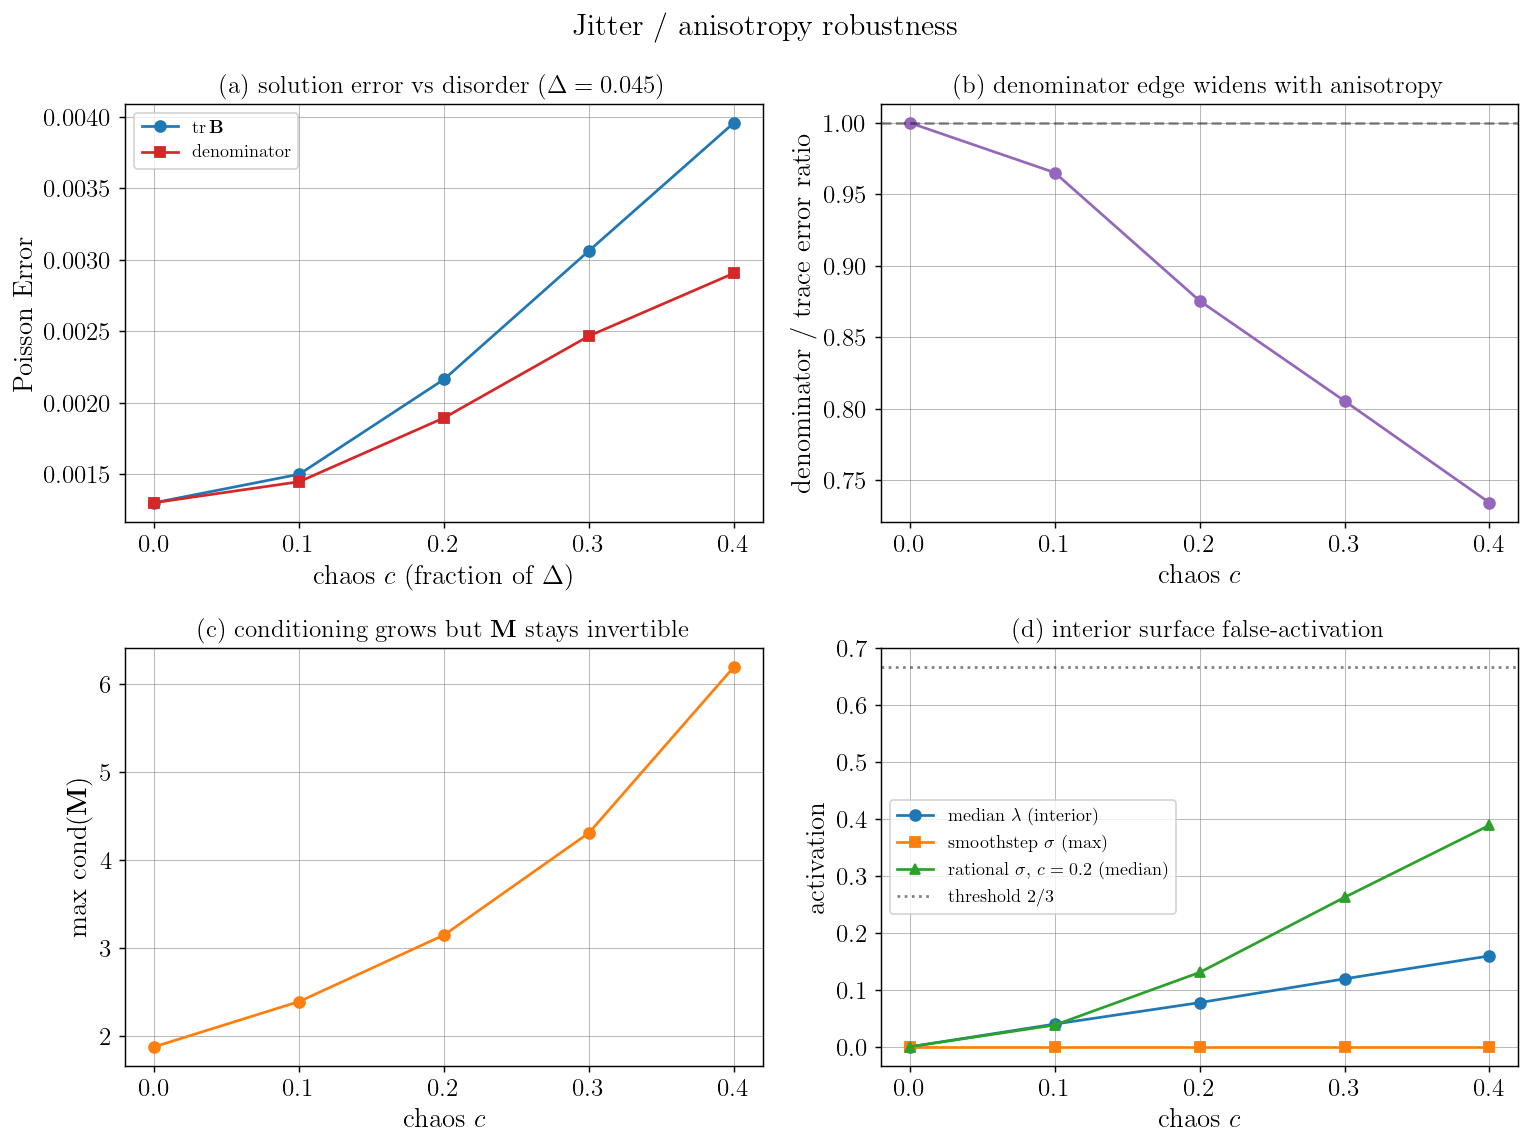
\includegraphics[width=\textwidth]{fig_jitter.png}
  \caption{Disorder robustness. (a) Poisson error against disorder for the two
  normalisations. (b) The denominator-to-trace error ratio narrowing with disorder. (c) The
  condition number of $\Mi$. (d) Interior surface false-activation, zero for the smoothstep and
  growing for a fixed-parameter rational activation.}
  \label{fig:jitter}
\end{figure}

% =============================================================================
\section{Application to the Helmholtz--Hodge decomposition}
\label{sec:hodge}

A natural application of the closure is the discrete Helmholtz--Hodge decomposition, in which a
vector field is split into a divergence-free part and the gradient of a scalar potential. The
pressure projection of an incompressible-flow solver is its best-known special case, but the
decomposition is generic and arises wherever a field must be projected onto its divergence-free
part; the treatment here is kept in those general terms. Given a vector field $\mathbf u^\ast$,
the decomposition $\mathbf u^\ast=\mathbf u+\nabla\phi$ with $\nabla\!\cdot\mathbf u=0$ is
computed by solving a scalar Poisson problem for the potential and subtracting its gradient,
\begin{equation}
  \mathsf L\,\phi=\langle\nabla\!\cdot\mathbf u^\ast\rangle,\qquad
  \mathbf u=\mathbf u^\ast-\gradop{\phi},
  \label{eq:projection}
\end{equation}
where $\mathsf L$ is the renormalised Laplacian with the boundary closure of
Section~\ref{sec:closure}, the divergence
$\langle\nabla\!\cdot\mathbf u^\ast\rangle_i=\sum_c\mathbf e_c\cdot\gradop{u^\ast_c}_i$ is the
trace of the component-wise renormalised gradient~\eqref{eq:grad}, and the potential satisfies a
Neumann condition at a wall and a value condition at a free surface, by the
boundary-condition-by-type principle of Section~\ref{sec:closure}. A concern specific to a
meshless, collocated discretisation is that the operators are not mutually adjoint: the
single-sum Laplacian~\eqref{eq:lap} is not the composition of the discrete divergence and
gradient, $\mathsf L\neq\mathsf D\mathsf G$, where $\mathsf D$ and $\mathsf G$ denote the
divergence and gradient matrices. Subtracting the gradient therefore does not annihilate the
divergence exactly, and the residual divergence of the computed solenoidal part is, by
Eq.~\eqref{eq:projection},
\begin{equation}
  \langle\nabla\!\cdot\mathbf u\rangle
  =\langle\nabla\!\cdot\mathbf u^\ast\rangle-\mathsf D\mathsf G\,\phi
  =\mathsf L\phi-\mathsf D\mathsf G\,\phi
  =(\mathsf L-\mathsf D\mathsf G)\,\phi.
  \label{eq:projresidual}
\end{equation}
The residual divergence is exactly the operator commutation defect
$(\mathsf L-\mathsf D\mathsf G)$ applied to the computed potential. It vanishes identically for
a staggered finite-difference or finite-volume discretisation, for which
$\mathsf L=\mathsf D\mathsf G$ and the decomposition is exact, and is otherwise a measure of the
operators' non-adjointness. The question is whether this residual is small and whether it
vanishes under refinement.

A manufactured Helmholtz--Hodge decomposition provides an analytic ground truth. With a
stream function $\psi=\sin\pi x\,\sin\pi y$ and a potential $\phi^\star=\cos2\pi x\,\cos2\pi y$,
the field
\begin{equation}
  \mathbf u^\ast=\nabla^\perp\!\psi+\nabla\phi^\star,\qquad
  \nabla^\perp\!\psi=(\partial_y\psi,\,-\partial_x\psi),
  \label{eq:hodgefield}
\end{equation}
has the known divergence $\nabla\!\cdot\mathbf u^\ast=\nabla^2\phi^\star$, the exact potential
$\phi^\star$ up to a constant, and the exact divergence-free part $\nabla^\perp\!\psi$, which is
solenoidal by construction and tangential to the unit-box boundary since $\psi$ vanishes there.
The Neumann datum on a wall is the prescribed $\nabla\phi^\star\!\cdot\mathbf n$, so the
decomposition is exact on any domain, including the wedge tank of Section~\ref{sec:bvp}. The
discrete divergence $\langle\nabla\!\cdot\mathbf u^\ast\rangle$ is used as the source in
Eq.~\eqref{eq:projection}, as it would be in a solver, so that the identity~\eqref{eq:projresidual}
holds discretely.

Equation~\eqref{eq:projresidual} is confirmed to round-off, the directly measured residual
matching $(\mathsf L-\mathsf D\mathsf G)\phi$ to $\sim10^{-13}$ on the interior. A single
decomposition removes $80$ to $95\%$ of the divergence, and the residual converges under
refinement, at order $1.2$ on a regular lattice, $1.0$ on the wedge tank, and $0.4$ on the box
at chaos $60\%$ with the projection Neumann closure, mirroring the supraconvergent solution
orders of Section~\ref{sec:bvp}. The algebraic-ghost closure lowers the box residual by about a
third and sharply improves the recovered potential, raising its order from $0.9$ to $1.7$, but
it leaves the residual-divergence rate at about $0.4$, in contrast to the marked improvement it
brings to the Poisson solution rate in Section~\ref{sec:bvp}. That a better wall closure
improves the potential yet not the divergence rate is a first sign that the residual is limited
by the divergence--gradient pairing and not by the Laplacian closure, which the operator
comparison below makes precise. Figure~\ref{fig:hodge}(a) shows the residual against $\Delta$
for both closures on the box and for the wedge tank. The decomposition is
non-expansive, the solenoidal part carrying less energy than the field,
$\|\mathbf u\|/\|\mathbf u^\ast\|\approx0.47$, and the discrete inner product
$\langle\mathbf u,\gradop{\phi}\rangle$ between the two parts vanishes under refinement, so the
decomposition becomes orthogonal in the limit. The renormalised operators are therefore
consistent for a single decomposition: the residual divergence is precisely the non-adjointness
defect, and that defect vanishes as $\Delta\to0$.

The choice of Laplacian was then isolated. On an all-Dirichlet box, which every operator can
solve, the same renormalised gradient was used for $\mathsf D$ and $\mathsf G$ while the
Laplacian $\mathsf L$ in Eq.~\eqref{eq:projection} was varied across the uncorrected summation
$N_i\sum_j W_{ij}f_{ij}$, obtained by setting $w_{ij}=1$ in Eq.~\eqref{eq:lap}, the present
renormalised operator in its smooth-naive and sum normalisations, the GFDM operator of
Section~\ref{sec:bvp}, and the Full-Inverse operator of Asai et al.~\cite{Asai2023}.
Figure~\ref{fig:hodge}(c) reports the residual. The uncorrected summation diverges, its residual
growing under refinement, in keeping with the non-convergence of the classical uncorrected SPH
Laplacian on irregular clouds~\cite{Brookshaw1985,Fatehi2011,Basic2018}, so the renormalisation
correction is essential to projection consistency. The renormalised operator, the GFDM operator
and the Full-Inverse operator are by contrast all consistent and close, the two second-order
operators improving the residual only marginally over the linear-consistent renormalised one.
The reason is visible in Eq.~\eqref{eq:projresidual}: with a shared gradient the residual
$(\mathsf L-\mathsf D\mathsf G)\phi$ is set by the gradient pairing $\mathsf D\mathsf G$ and not
by the order of $\mathsf L$, so a more accurate Laplacian alone does not reduce it. Projection
consistency is thus a property of how the divergence and gradient are paired, more than of the
Laplacian's formal order, which is consistent with the central finding of this work that the
closure, and not the interior order, governs the realised accuracy.

The residual can be reduced further by repeating the decomposition, solving
Eq.~\eqref{eq:projection} for the current divergence and re-correcting. This defect correction
lowers the residual to a floor of about one to a few percent of the initial divergence, after
which it stalls, the asymptotic contraction factor approaching unity; the iteration does not
reach a divergence-free state, because the commutation defect has a near-null mode that it
cannot remove [Fig.~\ref{fig:hodge}(b)]. If the raw one-sided divergence at the wall nodes is
fed to the source rather than carried by the Neumann condition, the iteration diverges. This is
the flux-only Neumann limitation of Section~\ref{sec:closure} reappearing in the divergence of
the field, and it indicates that the divergence wall term is itself a candidate for the
algebraic-ghost completion. The renormalised closure is therefore suited to a single
Helmholtz--Hodge decomposition, where it gives a small residual divergence that vanishes under
refinement, rather than to an iteration towards an exactly divergence-free field.

\begin{figure}[t]
  \centering
  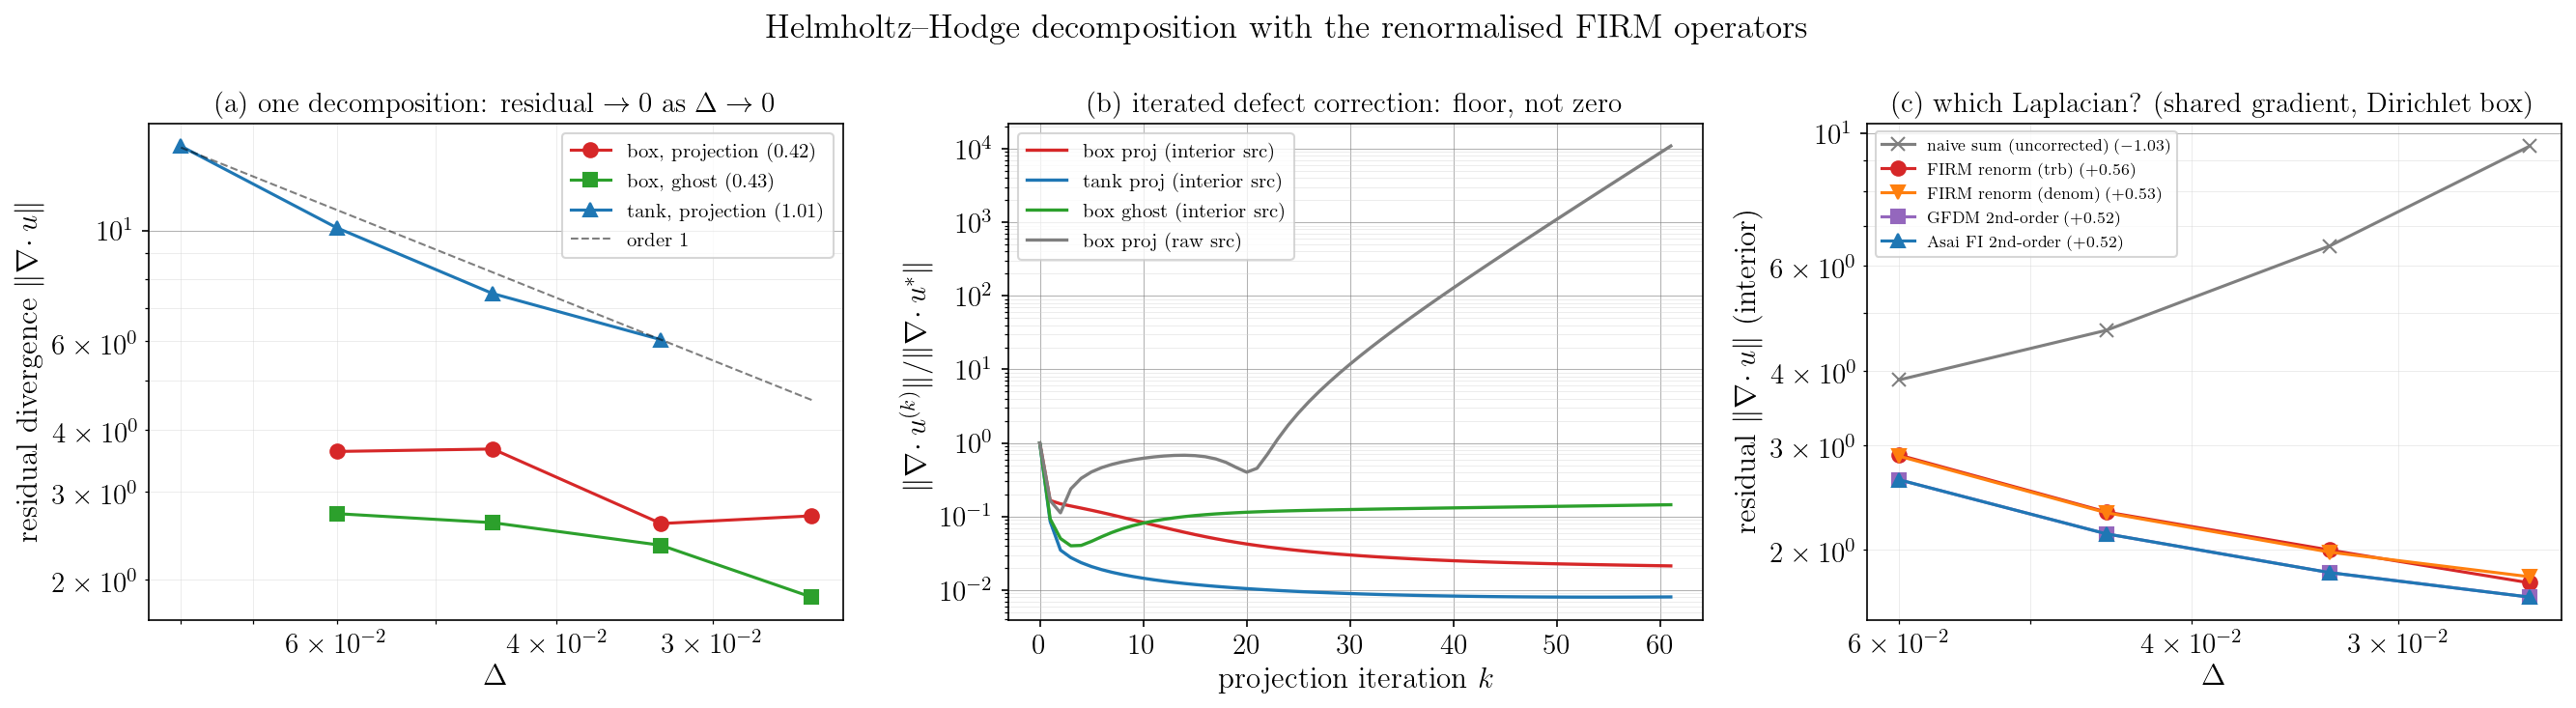
\includegraphics[width=\textwidth]{fig_hodge.png}
  \caption{The renormalised operators in a Helmholtz--Hodge decomposition of the manufactured
  field~\eqref{eq:hodgefield}. (a) The residual divergence of the solenoidal part after one
  decomposition against $\Delta$, on the box with the projection and algebraic-ghost Neumann
  closures and on the wedge tank, with an order-one reference; it vanishes under refinement.
  (b) Iterated defect correction at chaos $60\%$: the residual falls to a floor and stalls,
  while feeding the raw one-sided wall divergence to the source diverges. (c) The choice of
  Laplacian, with a shared gradient on a Dirichlet box: the uncorrected summation diverges,
  whereas the renormalised, GFDM and Full-Inverse operators are consistent and close, the
  residual being set by the gradient pairing rather than the Laplacian order.}
  \label{fig:hodge}
\end{figure}

% =============================================================================
\section{Discussion}
\label{sec:discussion}

\subsection{Computational aspects}
\label{sec:cost}

The closures add only local work to the interior assembly. The Neumann projection is a
$d\times d$ projector built from at most $K$ boundary normals, with a single $K\times K$ Gram
solve for GGP. The free-surface detection is the matrix-vector product $\Bi\ow$, already
available from the assembly. The algebraic-ghost closure appends at most a few image samples
per Neumann node and re-uses the same moment machinery. The boundary work is therefore $O(1)$
per boundary node and is incurred only on the $O(N^{(d-1)/d})$ boundary nodes. The assembled
system is sparse and nonsymmetric, because the correction weight $w_{ij}$ and the normalisation
$N_i$ are row-local, and a Krylov solver such as BiCGStab or QMR with a Jacobi or ILU(0)
preconditioner is appropriate, as in~\cite{Basic2018}. The recommended configuration is the
poly6 kernel at $h=2.5\Delta$, or $h\in[2.0,2.25]\Delta$ for quasi-uniform clouds, with GGP
projection for corner robustness and the algebraic-ghost closure where Neumann accuracy is
required. The choices of AN against GGP and of projection against ghost are isolated, local
code changes, since all downstream assembly consumes $\ow$ or the assembled row regardless.

\subsection{Operator and closure combinations}
\label{sec:combos}

Every node is a single row of Eq.~\eqref{eq:row}, so a scheme is just an interior Laplacian
together with a closure for each boundary type. Table~\ref{tab:schemes} collects the
combinations with their realised convergence orders and per-node cost. The diagonal closures
(projection, Robin) require the renormalised operator, whereas the reflection ghosts (even for a
Neumann flux, odd for a free surface) pair with any operator and may be mixed with the diagonal
forms, so the rows are representative rather than exhaustive. The smooth-naive and sum
normalisations of the renormalised operator give the same order with the diagonal closures, sum
only lowering the error constant, so the diagonal scheme is listed once; they differ only at the
even-ghost Neumann, where the sum normalisation (exact for $|\mathbf x|^2$) reaches about $1.8$
while smooth naive plateaus at about $1.4$, which is why both appear with the ghost closures.

\begin{table}[t]
  \centering
  \caption{Schemes for the unified row of Eq.~\eqref{eq:row}: an interior Laplacian with a
  Neumann and a free-surface closure, their realised solution-convergence orders (interior /
  Neumann / free surface) on disordered clouds, and relative per-node cost. ``smooth naive'' and
  ``sum'' are the trace- and denominator-normalised renormalised operators; ``ghost'' is the
  even/odd reflection closure. Orders from Sections~\ref{sec:bvp} and~\ref{sec:combos}; cost from
  Section~\ref{sec:cost}. The last column is the fraction of the field's divergence removed by a
  single Helmholtz--Hodge projection at the finest resolution tested (Section~\ref{sec:hodge},
  common renormalised gradient); being set by the divergence--gradient pairing rather than by the
  Laplacian, it reaches about the same value for every corrected scheme, the uncorrected operators
  alone failing to clean.}
  \label{tab:schemes}
  \small
  \begin{tabular}{@{}lllclc@{}}
    \toprule
    Laplacian & Neumann & Free surface & order (int / Neu / surf) & cost & div.\ cleaned \\
    \midrule
    smooth naive & projection & Robin & $1.4 / 0.9 / 1.8$ & lowest   & $94\%$ \\
    smooth naive & ghost      & ghost & $1.4 / 1.4 / 2.0$ & low      & $94\%$ \\
    sum          & ghost      & ghost & $1.4 / 1.8 / 2.0$ & low      & $94\%$ \\
    GFDM         & constraint & ghost & $1.8 / 0.9 / 2.0$ & high     & $94\%$ \\
    Full Inverse & ghost      & ghost & $1.8 / 1.8 / 2.0$ & moderate & $94\%$ \\
    \bottomrule
  \end{tabular}
\end{table}

Two of the table's rows are not, strictly, instances of the unified row, and the exceptions are
worth stating. The generalised finite difference operator does not fold the boundary into a
single equation: a Dirichlet node is pinned to its value and a Neumann node carries a local
Karush--Kuhn--Tucker constraint block, so its system mixes interior, pinned and constrained row
types. The Full-Inverse operator keeps one row per node, but that row is the solution of a
per-node least-squares system rather than the single renormalised sum of Eq.~\eqref{eq:row}.
Both are still free of boundary particles and of extra global unknowns --- the reflection ghost
is ephemeral and the constraint multiplier is eliminated locally --- yet neither is the
boundary-integrated single-equation form, and so neither is FIRM proper: they enter the table as
a second-order interior baseline (GFDM) and as the same-family second-order operator (Full
Inverse) that the algebraic-ghost closure is shown to transfer to, not as instances of the
method. Canonical FIRM is the renormalised operator with the boundary flux integrated into the
operator itself --- the Neumann flux placed in the right-hand side, and the free-surface value,
recast as the value-dependent Robin flux of Section~\ref{sec:surface}, split between the
right-hand side and the diagonal of one and the same row, with no boundary nodes, no constraints
and no auxiliary unknowns. That is the first row of Table~\ref{tab:schemes}, the smooth-naive operator with the
projection and Robin closures, of which the ghost rows are the stencil-completing variant, and
which the name denotes exactly: a flux-integrated renormalised meshless operator.

Two practical messages follow from Table~\ref{tab:schemes}. The renormalised operators
introduced here are not the most accurate available: a fully second-order interior, whether the
GFDM least-squares operator or the same-family Full-Inverse operator of Asai et
al.~\cite{Asai2023}, attains a higher interior order. What the present construction offers
instead is convenience. The interior operator is a single neighbour loop with no local linear
solve, the boundary conditions are integrated by type on one code path with no auxiliary
unknowns and no tuning, and the reflection-ghost closure is operator-agnostic, so a scheme is
assembled by choosing one row and one closure per boundary type rather than by deriving a new
operator. The cheapest combination in Table~\ref{tab:schemes}, the smooth-naive operator with
the projection and Robin closures, is also the simplest to implement.

The Helmholtz--Hodge decomposition sharpens this point. The realised cleaning of the divergence
is essentially independent of the accuracy ordering: every corrected scheme in
Table~\ref{tab:schemes}, from the low-order renormalised operator to the second-order GFDM and
Full-Inverse operators, removes the same $94\%$ of the field's divergence in a single
decomposition, because the residual is set by the divergence--gradient pairing and not by the
interior order (Section~\ref{sec:hodge}). The simple, low-order operator is therefore as
effective as the higher-accuracy operators for this purpose, at a fraction of the cost, and the
small remaining residual is reduced further by iterating the decomposition, which drives the
divergence down to a floor of about one percent. A low-order but conveniently assembled
operator, combined appropriately and applied iteratively, thus performs the Helmholtz--Hodge
decomposition on a par with the higher-order alternatives.

% =============================================================================
\section{Conclusions}
\label{sec:concl}

A boundary-integrated closure for renormalised meshless operators on elliptic boundary value
problems has been presented.
First, boundary conditions are integrated by type on a single code path. A Neumann flux enters
the right-hand side, a Dirichlet or Robin value enters the diagonal, and the interior, the
Neumann boundary, the free surface and the contact lines are assembled by one kernel. Second,
the Neumann condition is imposed by a tangential projection performed in physical space before
renormalisation, with a general Gram projector that treats arbitrary non-orthogonal corners
exactly, and a complementary algebraic-ghost closure that completes the truncated boundary
stencil without additional unknowns and removes the Neumann accuracy bottleneck. Third, the
free surface is detected from the support-deficiency geometry of the cloud and enforced without
any tuning or threshold parameter, the enforcement strength cancelling to the total kernel
weight.

The closures are linear-exact on any cloud, including truncated and corner rows, as verified
to round-off, and they were tested on irregular-domain Poisson benchmarks for regular and
highly irregular clouds against a second-order GFDM baseline. The convergence is reported in
full. The renormalised interior operator is linear-consistent and supraconverges at order
about $1.3$ under strong disorder, where a fully second-order GFDM operator is more accurate.
The value closure supraconverges, the flux-only Neumann closure is the accuracy-limiter, and
the algebraic-ghost closure reduces the Neumann-limited error by about an order of magnitude
and lets the Neumann region converge at the interior rate, approaching second order at a
straight boundary with the sum normalisation. The value of the method lies in the generality,
robustness and absence of tuning of its boundary closure, and in the convenience of its
assembly, rather than in a high formal order. The interior operator is a single neighbour loop
without a local solve, and the closures are selected by boundary type on one code path, so a
scheme is assembled by combination rather than by deriving a new operator (Table~\ref{tab:schemes}).

Several applications and extensions are topics for future work. The boundary closure is
generic for elliptic boundary value problems on moving point clouds. A leading application is
the Helmholtz--Hodge decomposition, examined in Section~\ref{sec:hodge}, in which the Neumann
condition arises at solid boundaries and the free surface carries the value condition, with the
pressure projection of an incompressible flow as one special case. There the operators are shown
to be consistent for a single decomposition, with the residual divergence equal to their
non-adjointness defect and vanishing under refinement, and governed by the divergence--gradient
pairing rather than the Laplacian order. In consequence the simple low-order operator cleans the
same fraction of the divergence in a single decomposition as the second-order GFDM and
Full-Inverse operators, and an iterated decomposition reduces the residual further, so the
conveniently assembled low-order construction performs the Helmholtz--Hodge decomposition on a
par with the higher-accuracy alternatives (Table~\ref{tab:schemes}). A full incompressible-flow
application would
additionally require the no-slip velocity Robin condition and the stress-free surface, which
inherit the same boundary-condition-by-type treatment, and a divergence-free time integration;
these were not assessed here. The motivating application is incompressible free-surface
hydrodynamics --- sloshing, dam break, and wave impact on moving point clouds --- where the
cloud-detected free surface, requiring neither surface particles nor a threshold, is the
principal advantage. A distinct near-term application is the processing of scattered experimental
velocity fields: pressure reconstruction from particle image velocimetry, in which a pressure
Poisson problem is solved on a masked, mesh-unfriendly domain with Neumann data from the momentum
balance at solid boundaries and a value condition at a free surface or far field, and the
Helmholtz--Hodge filtering of noisy measured fields onto their divergence-free part.
Fluid--structure interaction and other moving-boundary problems are further candidates for the
same Lagrangian, geometry-detected treatment. A locally second-order-consistent
interior operator, such as the Full-Inverse renormalised operator of Asai et
al.~\cite{Asai2023} that reinstates the cross-derivative coupling, lifts the whole-domain order.
Paired with the reflection-ghost closure --- even reflection for a Neumann wall, odd reflection
for a Dirichlet free surface, the two composed at a contact line --- which transfers unchanged
because it is operator-agnostic stencil completion, it yields about second order throughout: a
second-order interior, a Neumann boundary at order about $1.8$, a detected curved free surface
at order about $2.0$, and contact lines at the interior rate, with no extra unknowns
(Section~\ref{sec:combos}). The same reflection ghosts apply to the linear-consistent
renormalised operator, where the odd-ghost free surface in fact surpasses its diagonal-Robin
value closure. A high-order flux-only Neumann treatment through the staggered KKT
construction of Trask et al.~\cite{Trask2017} or the GFDM constraint
row~\cite{Kuhnert2001,Tiwari2003} remains for future work. A curvature-aware reflection (the
local planes are flat facets here), surface tension
through a meshless curvature estimate, and three-dimensional validation are also left for
future study.

% =============================================================================
\section*{Acknowledgements}
Placeholder.

\bibliographystyle{elsarticle-num}
\bibliography{firm}

\end{document}
